\documentclass[8pt,aspectratio=169]{beamer}
\usetheme{Madrid}
\usepackage{graphicx,booktabs,adjustbox,multicol,amsmath,listings,xcolor}
\definecolor{mlblue}{RGB}{0,102,204}
\definecolor{mlpurple}{RGB}{51,51,178}
\definecolor{mllavender}{RGB}{173,173,224}
\definecolor{mllavender2}{RGB}{193,193,232}
\definecolor{mllavender3}{RGB}{204,204,235}
\definecolor{mllavender4}{RGB}{214,214,239}
\definecolor{mlorange}{RGB}{255,127,14}
\definecolor{mlgreen}{RGB}{44,160,44}
\definecolor{mlred}{RGB}{214,39,40}
\definecolor{mlgray}{RGB}{127,127,127}
\setbeamercolor{palette primary}{bg=mllavender3,fg=mlpurple}
\setbeamercolor{palette secondary}{bg=mllavender2,fg=mlpurple}
\setbeamercolor{palette tertiary}{bg=mllavender,fg=white}
\setbeamercolor{palette quaternary}{bg=mlpurple,fg=white}
\setbeamercolor{structure}{fg=mlpurple}
\setbeamercolor{title}{fg=mlpurple}
\setbeamercolor{frametitle}{fg=mlpurple,bg=mllavender3}
\setbeamercolor{block title}{bg=mllavender2,fg=mlpurple}
\setbeamercolor{block body}{bg=mllavender4,fg=black}
\setbeamertemplate{navigation symbols}{}
\setbeamertemplate{itemize items}[circle]
\setbeamersize{text margin left=5mm,text margin right=5mm}
\newcommand{\bottomnote}[1]{\vfill\vspace{-2mm}\textcolor{mllavender2}{\rule{\textwidth}{0.4pt}}\vspace{1mm}\footnotesize\textbf{#1}}
\lstdefinestyle{python}{language=Python,basicstyle=\ttfamily\tiny,keywordstyle=\color{mlblue}\bfseries,stringstyle=\color{mlgreen},commentstyle=\color{mlgray}\itshape,frame=single,backgroundcolor=\color{mllavender4},breaklines=true,tabsize=4,showstringspaces=false}
\lstset{style=python}
\usepackage{tikz,pgfplots}
\pgfplotsset{compat=1.18}
\usetikzlibrary{arrows.meta,positioning,shapes.geometric,calc,chains,decorations.pathmorphing,automata}
\title{Blockchain Fundamentals: A Quantitative Deep Dive}
\subtitle{Standalone Technical Lecture}
\author{Prof.~Dr.~Joerg Osterrieder}
\institute{University Lecture Series}
\date{\today}
\begin{document}

%--- FRAME 1: Title ---
\begin{frame}
\titlepage
\end{frame}

\section{Introduction and Motivation}

%--- FRAME 2: Historical Timeline ---
\begin{frame}{Historical Timeline of Blockchain}
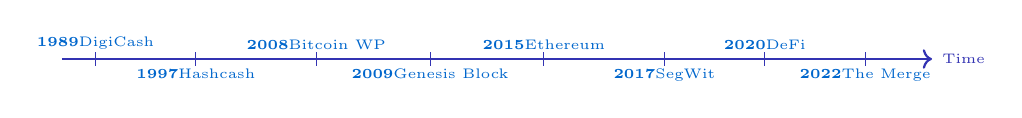
\begin{tikzpicture}[scale=0.85]
  \draw[->,thick,mlpurple] (0,0) -- (13,0) node[right]{\tiny Time};
  \foreach \x/\yr/\pos/\lbl in {
    0.5/1989/above/DigiCash,
    2.0/1997/below/Hashcash,
    3.8/2008/above/Bitcoin WP,
    5.5/2009/below/Genesis Block,
    7.2/2015/above/Ethereum,
    9.0/2017/below/SegWit,
    10.5/2020/above/DeFi,
    12.0/2022/below/The Merge}{
    \draw[mlpurple] (\x,0.1)--(\x,-0.1);
    \node[\pos,font=\tiny,mlblue,align=center] at (\x,0) {\textbf{\yr}\lbl};
  }
\end{tikzpicture}
\vspace{1mm}
\begin{columns}
\column{0.48\textwidth}
\begin{block}{Foundations}
\begin{itemize}\small
  \item \textbf{1989}: DigiCash -- blind signatures (Chaum)
  \item \textbf{1997}: Hashcash -- proof-of-work for spam
  \item \textbf{2008}: Bitcoin whitepaper (Satoshi Nakamoto)
  \item \textbf{2009}: Genesis block mined, first BTC tx
\end{itemize}
\end{block}
\column{0.48\textwidth}
\begin{block}{Modern Era}
\begin{itemize}\small
  \item \textbf{2015}: Ethereum -- Turing-complete contracts
  \item \textbf{2017}: SegWit fixes transaction malleability
  \item \textbf{2020}: DeFi summer, TVL exceeds \$10B
  \item \textbf{2022}: Ethereum transitions to Proof of Stake
\end{itemize}
\end{block}
\end{columns}
\bottomnote{35 years: from theoretical digital cash to global financial infrastructure}
\end{frame}

%--- FRAME 3: Double-Spending Problem ---
\begin{frame}{The Double-Spending Problem}
\begin{columns}
\column{0.44\textwidth}
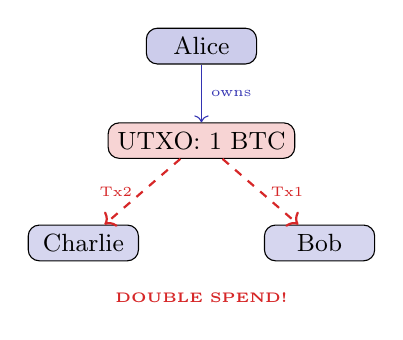
\begin{tikzpicture}[font=\small]
  \node[draw,fill=mllavender3,rounded corners,minimum width=1.4cm] (alice) at (1.5,3.2) {Alice};
  \node[draw,fill=mlred!20,rounded corners,minimum width=1.8cm] (utxo) at (1.5,2.0) {UTXO: 1 BTC};
  \node[draw,fill=mllavender4,rounded corners,minimum width=1.4cm] (bob) at (3.0,0.7) {Bob};
  \node[draw,fill=mllavender4,rounded corners,minimum width=1.4cm] (charlie) at (0.0,0.7) {Charlie};
  \draw[->,mlpurple] (alice)--(utxo) node[midway,right,font=\tiny]{owns};
  \draw[->,mlred,thick,dashed] (utxo)--(bob) node[midway,right,font=\tiny]{Tx1};
  \draw[->,mlred,thick,dashed] (utxo)--(charlie) node[midway,left,font=\tiny]{Tx2};
  \node[font=\tiny,mlred] at (1.5,0.0) {\textbf{DOUBLE SPEND!}};
\end{tikzpicture}
\column{0.54\textwidth}
\begin{block}{Formal Invariant}
Let $\mathcal{U}$ be the UTXO set. The double-spend invariant requires:
\[\forall\, u \in \mathcal{U}:\;\sum_{\substack{T:\,u\in\mathrm{inputs}(T)}} \mathbf{1}[\mathrm{conf}(T)] \leq 1\]
Each output may be consumed \textbf{at most once}.
\end{block}
\vspace{2mm}
\begin{block}{Why Difficult Without Central Authority?}
\begin{itemize}\small
  \item Network latency: conflicting txs arrive in different order at different nodes
  \item Sybil nodes selectively relay or suppress messages
  \item No global clock for deterministic ordering
\end{itemize}
\end{block}
\begin{alertblock}{Solution}
\small Nakamoto consensus: longest-chain rule with cumulative PoW defines canonical ordering.
\end{alertblock}
\end{columns}
\bottomnote{Bitcoin solves double-spending without any trusted third party for the first time}
\end{frame}

%--- FRAME 4: Trust Models ---
\begin{frame}{Trust Models: Centralized vs.\ Decentralized}
\begin{columns}
\column{0.46\textwidth}
\centering\small\textbf{Centralized (Bank)}\\[4pt]
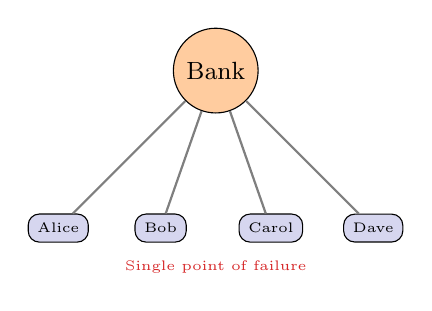
\begin{tikzpicture}
  \node[draw,circle,fill=mlorange!40,font=\small,minimum size=1cm] (bank) at (2.0,2.0) {Bank};
  \node[draw,fill=mllavender4,rounded corners,font=\tiny] (u1) at (0,0) {Alice};
  \node[draw,fill=mllavender4,rounded corners,font=\tiny] (u2) at (1.3,0) {Bob};
  \node[draw,fill=mllavender4,rounded corners,font=\tiny] (u3) at (2.7,0) {Carol};
  \node[draw,fill=mllavender4,rounded corners,font=\tiny] (u4) at (4.0,0) {Dave};
  \foreach \u in {u1,u2,u3,u4}{\draw[mlgray,thick] (\u)--(bank);}
  \node[font=\tiny,mlred] at (2.0,-0.5) {Single point of failure};
\end{tikzpicture}
\column{0.46\textwidth}
\centering\small\textbf{Decentralized (P2P)}\\[4pt]
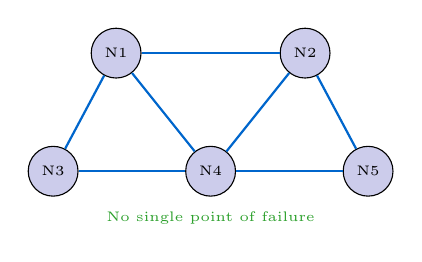
\begin{tikzpicture}
  \node[draw,circle,fill=mllavender3,font=\tiny] (n1) at (0.8,2.0) {N1};
  \node[draw,circle,fill=mllavender3,font=\tiny] (n2) at (3.2,2.0) {N2};
  \node[draw,circle,fill=mllavender3,font=\tiny] (n3) at (0,0.5) {N3};
  \node[draw,circle,fill=mllavender3,font=\tiny] (n4) at (2.0,0.5) {N4};
  \node[draw,circle,fill=mllavender3,font=\tiny] (n5) at (4.0,0.5) {N5};
  \foreach \a/\b in {1/2,1/3,1/4,2/4,2/5,3/4,4/5}{\draw[mlblue,thick] (n\a)--(n\b);}
  \node[font=\tiny,mlgreen] at (2.0,-0.1) {No single point of failure};
\end{tikzpicture}
\end{columns}
\vspace{3mm}
\begin{columns}
\column{0.48\textwidth}
\begin{block}{Centralized}\small
Fast, simple, regulated. But: censorable, single failure point, requires trust.
\end{block}
\column{0.48\textwidth}
\begin{block}{Decentralized}\small
Trustless, Byzantine fault tolerant, censorship-resistant. But: slower, complex.
\end{block}
\end{columns}
\bottomnote{Blockchain replaces institutional trust with cryptographic and game-theoretic guarantees}
\end{frame}

%--- FRAME 5: Roadmap ---
\begin{frame}{Lecture Roadmap}
\begin{columns}
\column{0.5\textwidth}
\begin{block}{8 Sections}
\begin{enumerate}\small
  \item \textcolor{mlpurple}{\textbf{Introduction \& Motivation}} \checkmark
  \item \textbf{Block Anatomy} -- structure, UTXO, accounts
  \item \textbf{Hash Functions} -- SHA-256, properties
  \item \textbf{Merkle Trees} -- SPV proofs, tries
  \item \textbf{Proof of Work} -- mining, difficulty, energy
  \item \textbf{Proof of Stake} -- validators, Casper FFG
  \item \textbf{Network} -- P2P, propagation, forks
  \item \textbf{Security \& Future} -- attacks, L2, quantum
\end{enumerate}
\end{block}
\column{0.46\textwidth}
\begin{block}{Learning Objectives}
\begin{itemize}\small
  \item Master blockchain data structures
  \item Derive mining difficulty mathematics
  \item Compare PoW vs.\ PoS security models
  \item Analyze network-level attack vectors
  \item Quantify decentralization with metrics
\end{itemize}
\end{block}
\vspace{2mm}
\begin{alertblock}{Central Question}
\small How do mutually distrusting parties reach consensus on a shared ledger history?
\end{alertblock}
\end{columns}
\bottomnote{Prerequisites: probability theory, basic cryptography, graph theory}
\end{frame}

\begin{frame}{Learning Objectives}
By the end of this lecture, you will be able to:
\begin{enumerate}
\item \textbf{Explain} the double-spending problem and how blockchain provides a trustless solution
\item \textbf{Describe} the internal structure of a block (header, body, Merkle root, hash pointers)
\item \textbf{Compare} Proof of Work and Proof of Stake consensus mechanisms quantitatively
\item \textbf{Analyze} the security guarantees of hash-chain immutability and collision resistance
\item \textbf{Evaluate} trade-offs in the blockchain trilemma (scalability, security, decentralization)
\end{enumerate}
\bottomnote{Bloom's taxonomy levels: Remember $\rightarrow$ Understand $\rightarrow$ Apply $\rightarrow$ Analyze $\rightarrow$ Evaluate $\rightarrow$ Create}
\end{frame}

\section{Block Anatomy}

%--- FRAME 6: Block Data Structure ---
\begin{frame}{Block Data Structure}
\begin{columns}
\column{0.5\textwidth}
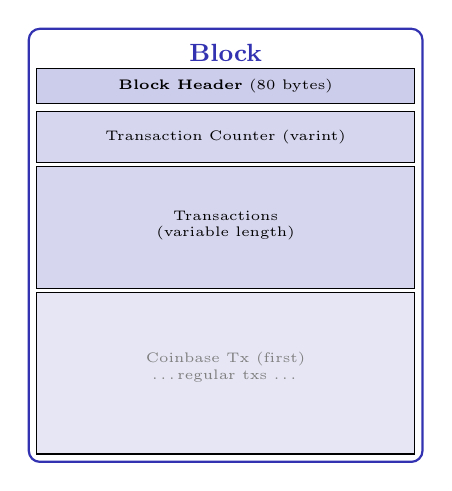
\begin{tikzpicture}[font=\small]
  \draw[mlpurple,thick,rounded corners] (0,0) rectangle (5,5.5);
  \node[mlpurple,font=\small\bfseries] at (2.5,5.2) {Block};
  \draw[fill=mllavender3] (0.1,4.55) rectangle (4.9,5.0);
  \node[font=\tiny] at (2.5,4.77) {\textbf{Block Header} (80 bytes)};
  \draw[fill=mllavender4] (0.1,3.8) rectangle (4.9,4.45);
  \node[font=\tiny] at (2.5,4.12) {Transaction Counter (varint)};
  \draw[fill=mllavender4] (0.1,2.2) rectangle (4.9,3.75);
  \node[font=\tiny,align=center] at (2.5,3.0) {Transactions\\(variable length)};
  \draw[fill=mllavender3!50] (0.1,0.1) rectangle (4.9,2.15);
  \node[font=\tiny,align=center,mlgray] at (2.5,1.2) {Coinbase Tx (first)\\\ldots regular txs \ldots};
\end{tikzpicture}
\column{0.48\textwidth}
\begin{block}{Key Fields \& Sizes}
\begin{tabular}{lll}
\toprule
\textbf{Field} & \textbf{Size} & \textbf{Notes}\\
\midrule
Magic bytes & 4 B & \texttt{0xD9B4BEF9}\\
Block size & 4 B & bytes following\\
Header & 80 B & fixed\\
Tx count & 1--9 B & varint\\
Txns & var & coinbase first\\
\bottomrule
\end{tabular}
\end{block}
\vspace{2mm}
\begin{block}{Block Size Limits}
\begin{itemize}\small
  \item Bitcoin: 1 MB legacy / 4 MB weight
  \item Ethereum: target 15M gas / max 30M
  \item Larger blocks: more TPS, higher orphan rate
\end{itemize}
\end{block}
\end{columns}
\bottomnote{Bitcoin average block $\approx$1.5 MB; $\approx$2500 transactions; mined every 10 minutes}
\end{frame}

%--- FRAME 7: Block Header ---
\begin{frame}{Block Header: 80 Bytes}
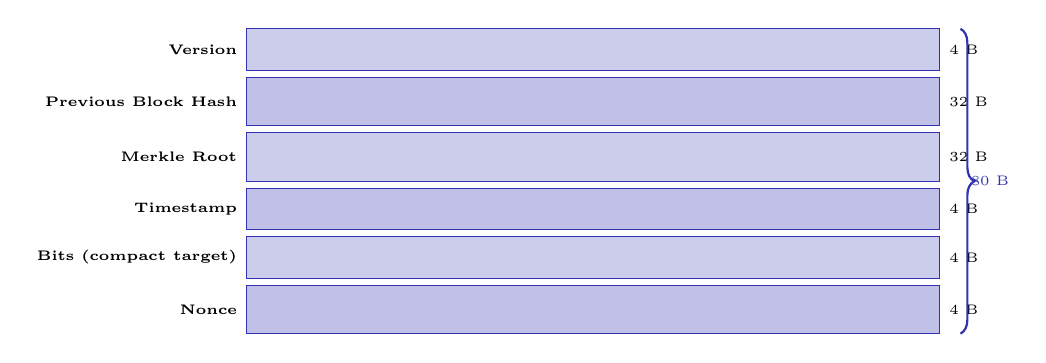
\begin{tikzpicture}[scale=0.88]
  \draw[fill=mllavender3,draw=mlpurple] (0,4.2) rectangle (10,4.8);
  \node[font=\tiny,left] at (0,4.5) {\textbf{Version}};
  \node[font=\tiny,right] at (10,4.5) {4 B};
  \draw[fill=mllavender2,draw=mlpurple] (0,3.4) rectangle (10,4.1);
  \node[font=\tiny,left] at (0,3.75) {\textbf{Previous Block Hash}};
  \node[font=\tiny,right] at (10,3.75) {32 B};
  \draw[fill=mllavender3,draw=mlpurple] (0,2.6) rectangle (10,3.3);
  \node[font=\tiny,left] at (0,2.95) {\textbf{Merkle Root}};
  \node[font=\tiny,right] at (10,2.95) {32 B};
  \draw[fill=mllavender2,draw=mlpurple] (0,1.9) rectangle (10,2.5);
  \node[font=\tiny,left] at (0,2.2) {\textbf{Timestamp}};
  \node[font=\tiny,right] at (10,2.2) {4 B};
  \draw[fill=mllavender3,draw=mlpurple] (0,1.2) rectangle (10,1.8);
  \node[font=\tiny,left] at (0,1.5) {\textbf{Bits (compact target)}};
  \node[font=\tiny,right] at (10,1.5) {4 B};
  \draw[fill=mllavender2,draw=mlpurple] (0,0.4) rectangle (10,1.1);
  \node[font=\tiny,left] at (0,0.75) {\textbf{Nonce}};
  \node[font=\tiny,right] at (10,0.75) {4 B};
  \draw[decorate,decoration={brace,amplitude=5pt},mlpurple,thick] (10.3,4.8)--(10.3,0.4) node[midway,right,font=\tiny,mlpurple]{80 B};
\end{tikzpicture}
\vspace{2mm}
\begin{columns}
\column{0.48\textwidth}
\begin{block}{Field Roles}\small
\begin{itemize}
  \item \textbf{prevHash}: creates chain linkage
  \item \textbf{merkleRoot}: commits to all transactions
  \item \textbf{bits}: compact form of target $T$
  \item \textbf{nonce}: miner iterates this field
\end{itemize}
\end{block}
\column{0.48\textwidth}
\begin{block}{Compact Target Decoding}\small
\[T = \texttt{coeff} \times 256^{(\texttt{exp}-3)}\]
Mining succeeds when:
\[\text{SHA256}^2(\text{header}) < T\]
\end{block}
\end{columns}
\bottomnote{Header hashed twice (double-SHA256); nonce space $2^{32}=4$B gives $\sim$4 GH per nonce cycle}
\end{frame}

%--- FRAME 8: UTXO Model ---
\begin{frame}{The UTXO Model}
\begin{columns}
\column{0.55\textwidth}
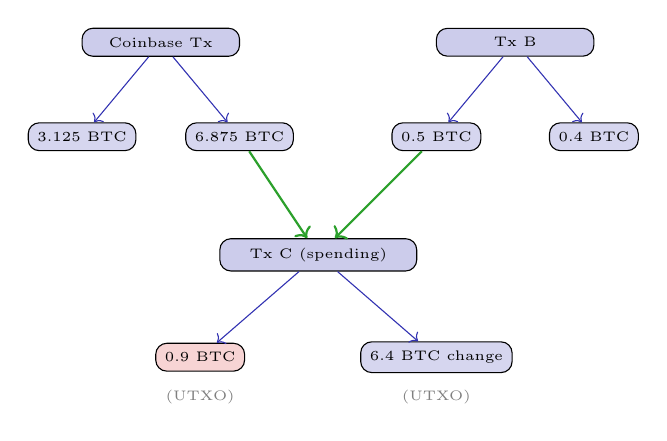
\begin{tikzpicture}[font=\tiny]
  \node[draw,fill=mllavender3,rounded corners,minimum width=2cm] (tx1) at (0.5,4.2) {Coinbase Tx};
  \node[draw,fill=mllavender4,rounded corners] (o1) at (-0.5,3.0) {3.125 BTC};
  \node[draw,fill=mllavender4,rounded corners] (o2) at (1.5,3.0) {6.875 BTC};
  \draw[->,mlpurple] (tx1)--(o1);
  \draw[->,mlpurple] (tx1)--(o2);
  \node[draw,fill=mllavender3,rounded corners,minimum width=2cm] (tx2) at (5.0,4.2) {Tx B};
  \node[draw,fill=mllavender4,rounded corners] (o3) at (4.0,3.0) {0.5 BTC};
  \node[draw,fill=mllavender4,rounded corners] (o4) at (6.0,3.0) {0.4 BTC};
  \draw[->,mlpurple] (tx2)--(o3);
  \draw[->,mlpurple] (tx2)--(o4);
  \node[draw,fill=mllavender3,rounded corners,minimum width=2.5cm] (tx3) at (2.5,1.5) {Tx C (spending)};
  \draw[->,mlgreen,thick] (o2)--(tx3);
  \draw[->,mlgreen,thick] (o3)--(tx3);
  \node[draw,fill=mlred!20,rounded corners] (o5) at (1.0,0.2) {0.9 BTC};
  \node[draw,fill=mllavender4,rounded corners] (o6) at (4.0,0.2) {6.4 BTC change};
  \draw[->,mlpurple] (tx3)--(o5);
  \draw[->,mlpurple] (tx3)--(o6);
  \node[mlgray,font=\tiny] at (1.0,-0.3) {(UTXO)};
  \node[mlgray,font=\tiny] at (4.0,-0.3) {(UTXO)};
\end{tikzpicture}
\column{0.42\textwidth}
\begin{block}{UTXO Properties}
\begin{itemize}\small
  \item Each output is atomic (no partial spend)
  \item Once spent, removed from UTXO set
  \item New outputs added when tx confirmed
  \item UTXO set fits in RAM ($\approx$4 GB)
\end{itemize}
\end{block}
\vspace{2mm}
\begin{block}{Conservation Law}
\[\sum_{\text{in}} v_i \geq \sum_{\text{out}} v_j\]
Difference = miner fee (implicitly claimed by coinbase)
\end{block}
\end{columns}
\bottomnote{Bitcoin UTXO set: $\approx$4.5M entries (2024); stored in LevelDB on full nodes}
\end{frame}

%--- FRAME 9: Account Model ---
\begin{frame}{Ethereum Account Model}
\begin{columns}
\column{0.48\textwidth}
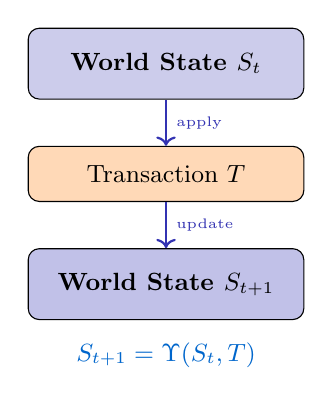
\begin{tikzpicture}[font=\small]
  \node[draw,fill=mllavender3,rounded corners,minimum width=3.5cm,minimum height=0.9cm] (s0) at (2,4.2) {\textbf{World State $S_t$}};
  \node[draw,fill=mlorange!30,rounded corners,minimum width=3.5cm,minimum height=0.7cm] (tx) at (2,2.8) {Transaction $T$};
  \node[draw,fill=mllavender2,rounded corners,minimum width=3.5cm,minimum height=0.9cm] (s1) at (2,1.4) {\textbf{World State $S_{t+1}$}};
  \draw[->,mlpurple,thick] (s0)--(tx) node[midway,right,font=\tiny]{apply};
  \draw[->,mlpurple,thick] (tx)--(s1) node[midway,right,font=\tiny]{update};
  \node[font=\small,mlblue] at (2,0.5) {$S_{t+1} = \Upsilon(S_t,T)$};
\end{tikzpicture}
\column{0.50\textwidth}
\begin{block}{Account State Fields}
\begin{tabular}{ll}
\toprule
\textbf{Field} & \textbf{Meaning}\\
\midrule
nonce & tx count (EOA) / deploys (contract)\\
balance & ETH in Wei\\
codeHash & keccak256(bytecode)\\
storageRoot & Patricia trie root\\
\bottomrule
\end{tabular}
\end{block}
\vspace{2mm}
\begin{block}{EOA vs.\ Contract Account}
\begin{itemize}\small
  \item \textbf{EOA}: codeHash = keccak256(\texttt{""}), no storage; controlled by private key
  \item \textbf{Contract}: deployed bytecode; triggered by messages; has persistent storage
\end{itemize}
\end{block}
\end{columns}
\bottomnote{State transition $\Upsilon$ defined in Ethereum Yellow Paper; gas limits computational cost}
\end{frame}

%--- FRAME 10: Transaction Structure ---
\begin{frame}{Bitcoin Transaction Anatomy}
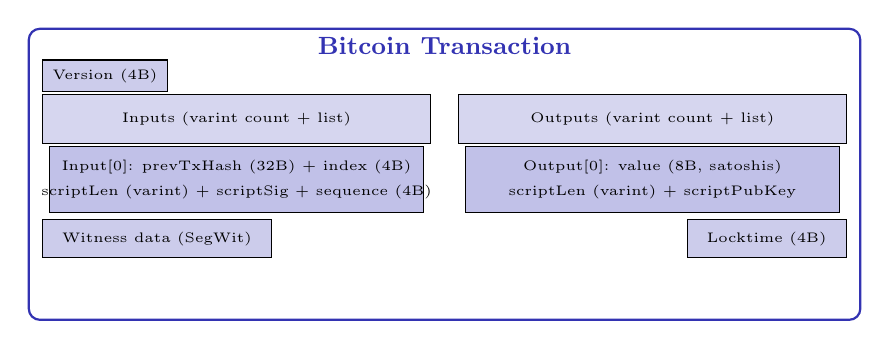
\begin{tikzpicture}[font=\tiny,scale=0.88]
  \draw[mlpurple,thick,rounded corners] (0,0) rectangle (12,4.2);
  \node[mlpurple,font=\small\bfseries] at (6,3.95) {Bitcoin Transaction};
  \draw[fill=mllavender3] (0.2,3.3) rectangle (2.0,3.75); \node at (1.1,3.52) {Version (4B)};
  \draw[fill=mllavender4] (0.2,2.55) rectangle (5.8,3.25); \node at (3.0,2.9) {Inputs (varint count + list)};
  \draw[fill=mllavender2] (0.3,1.55) rectangle (5.7,2.5);
  \node at (3.0,2.2) {Input[0]: prevTxHash (32B) + index (4B)};
  \node at (3.0,1.85) {scriptLen (varint) + scriptSig + sequence (4B)};
  \draw[fill=mllavender4] (6.2,2.55) rectangle (11.8,3.25); \node at (9.0,2.9) {Outputs (varint count + list)};
  \draw[fill=mllavender2] (6.3,1.55) rectangle (11.7,2.5);
  \node at (9.0,2.2) {Output[0]: value (8B, satoshis)};
  \node at (9.0,1.85) {scriptLen (varint) + scriptPubKey};
  \draw[fill=mllavender3] (0.2,0.9) rectangle (3.5,1.45); \node at (1.85,1.17) {Witness data (SegWit)};
  \draw[fill=mllavender3] (9.5,0.9) rectangle (11.8,1.45); \node at (10.65,1.17) {Locktime (4B)};
\end{tikzpicture}
\vspace{2mm}
\begin{columns}
\column{0.5\textwidth}
\begin{block}{Script Execution}\small
Stack-based. P2PKH scriptPubKey:\\
\texttt{OP\_DUP OP\_HASH160 <hash> OP\_EQUALVERIFY OP\_CHECKSIG}
\end{block}
\column{0.48\textwidth}
\begin{block}{Transaction ID}
\[\texttt{txid} = \text{SHA256}(\text{SHA256}(\text{raw bytes}))\]
SegWit: \texttt{wtxid} includes witness. Segwit discount: witness bytes cost 0.25 weight units.
\end{block}
\end{columns}
\bottomnote{Typical P2PKH tx $\approx$250 bytes; SegWit P2WPKH $\approx$141 vBytes (virtual bytes)}
\end{frame}

%--- FRAME 11: Coinbase Transaction ---
\begin{frame}{Coinbase Transaction \& Bitcoin Supply}
\begin{columns}
\column{0.48\textwidth}
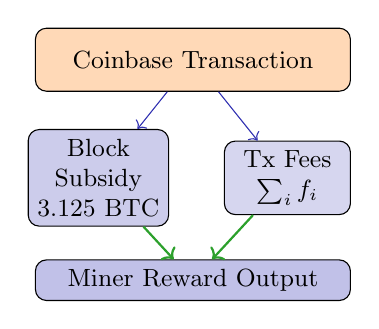
\begin{tikzpicture}[font=\small]
  \node[draw,fill=mlorange!30,rounded corners,minimum width=4cm,minimum height=0.8cm] (cb) at (2,3.5) {Coinbase Transaction};
  \node[draw,fill=mllavender3,rounded corners,minimum width=1.6cm,align=center] (sub) at (0.8,2.0) {Block\\Subsidy\\3.125 BTC};
  \node[draw,fill=mllavender4,rounded corners,minimum width=1.6cm,align=center] (fee) at (3.2,2.0) {Tx Fees\\$\sum_i f_i$};
  \draw[->,mlpurple] (cb)--(sub);
  \draw[->,mlpurple] (cb)--(fee);
  \node[draw,fill=mllavender2,rounded corners,minimum width=4cm] (miner) at (2,0.7) {Miner Reward Output};
  \draw[->,mlgreen,thick] (sub)--(miner);
  \draw[->,mlgreen,thick] (fee)--(miner);
\end{tikzpicture}
\column{0.50\textwidth}
\begin{block}{Halving Schedule}
\[R(n) = \frac{50}{2^n}\ \text{BTC},\quad n=\left\lfloor\frac{h}{210{,}000}\right\rfloor\]
\begin{tabular}{lll}
\toprule
Halving & Height & Reward\\
\midrule
0 & 0 & 50 BTC\\
1 & 210,000 & 25 BTC\\
3 & 630,000 & 6.25 BTC\\
4 & 840,000 & 3.125 BTC\\
\bottomrule
\end{tabular}
\end{block}
\vspace{1mm}
\begin{block}{Total Supply (Geometric Series)}
\[\sum_{n=0}^{\infty}210{,}000\cdot\frac{50}{2^n}=210{,}000\cdot100=21{,}000{,}000\ \text{BTC}\]
\end{block}
\end{columns}
\bottomnote{Last Bitcoin mined $\approx$2140; thereafter miners earn transaction fees only}
\end{frame}

\section{Hash Functions}

%--- FRAME 12: Hash Properties ---
\begin{frame}{Cryptographic Hash Function Properties}
\begin{block}{Definition}
A hash function $H:\{0,1\}^*\to\{0,1\}^n$ must satisfy three hardness properties:
\end{block}
\vspace{2mm}
\begin{columns}
\column{0.32\textwidth}
\begin{block}{1. Preimage Resistance}
Given $y$, hard to find $x$ s.t.\ $H(x)=y$.\\[4pt]
\small Security: $\mathcal{O}(2^n)$ work.\\[4pt]
\textit{``One-way function''}
\end{block}
\column{0.32\textwidth}
\begin{block}{2. Second Preimage}
Given $x$, hard to find $x'\neq x$ s.t.\ $H(x')=H(x)$.\\[4pt]
\small Security: $\mathcal{O}(2^n)$ work.\\[4pt]
\textit{``Weak collision''}
\end{block}
\column{0.32\textwidth}
\begin{block}{3. Collision Resistance}
Hard to find any $x\neq x'$ s.t.\ $H(x)=H(x')$.\\[4pt]
\small Security: $\mathcal{O}(2^{n/2})$ via birthday.\\[4pt]
\textit{``Strong collision''}
\end{block}
\end{columns}
\vspace{3mm}
\begin{columns}
\column{0.48\textwidth}
\begin{block}{SHA-256 Parameters}
\begin{itemize}\small
  \item Output: 256 bits = 32 bytes
  \item Block size: 512 bits
  \item Rounds: 64
  \item State: 8 $\times$ 32-bit words (256 bits)
\end{itemize}
\end{block}
\column{0.48\textwidth}
\begin{block}{Bitcoin Usage}
\begin{itemize}\small
  \item Block hash: SHA256$^2$(header)
  \item TXID: SHA256$^2$(raw tx)
  \item P2PKH: RIPEMD160(SHA256(pubkey))
  \item Merkle nodes: SHA256$^2$(left$\|$right)
\end{itemize}
\end{block}
\end{columns}
\bottomnote{SHA-256: NIST standard (2001); no practical collision known; 128-bit post-quantum security}
\end{frame}

%--- FRAME 13: SHA-256 Pipeline ---
\begin{frame}{SHA-256: Merkle--Damg\r{a}rd Construction}
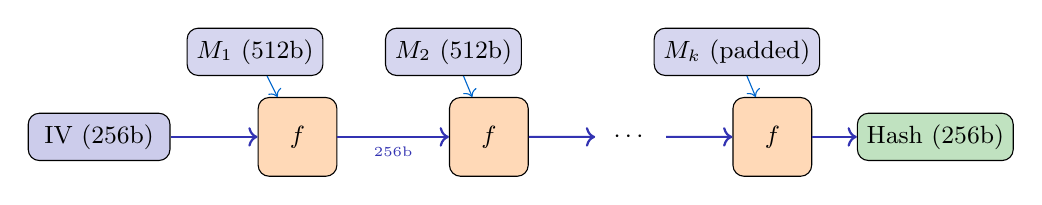
\begin{tikzpicture}[font=\small,scale=0.9]
  \node[draw,fill=mllavender3,rounded corners,minimum width=1.8cm,minimum height=0.6cm] (iv) at (0,2) {IV (256b)};
  \node[draw,fill=mllavender4,rounded corners,minimum width=1.2cm,minimum height=0.6cm] (m1) at (2.2,3.2) {$M_1$ (512b)};
  \node[draw,fill=mlorange!30,rounded corners,minimum width=1.0cm,minimum height=1.0cm] (c1) at (2.8,2) {$f$};
  \node[draw,fill=mllavender4,rounded corners,minimum width=1.2cm,minimum height=0.6cm] (m2) at (5.0,3.2) {$M_2$ (512b)};
  \node[draw,fill=mlorange!30,rounded corners,minimum width=1.0cm,minimum height=1.0cm] (c2) at (5.5,2) {$f$};
  \node[font=\small] at (7.5,2) {$\cdots$};
  \node[draw,fill=mllavender4,rounded corners,minimum width=1.2cm,minimum height=0.6cm] (mk) at (9.0,3.2) {$M_k$ (padded)};
  \node[draw,fill=mlorange!30,rounded corners,minimum width=1.0cm,minimum height=1.0cm] (ck) at (9.5,2) {$f$};
  \node[draw,fill=mlgreen!30,rounded corners,minimum width=1.8cm,minimum height=0.6cm] (out) at (11.8,2) {Hash (256b)};
  \draw[->,mlpurple,thick] (iv)--(c1);
  \draw[->,mlblue] (m1)--(c1);
  \draw[->,mlpurple,thick] (c1)--(c2) node[midway,below,font=\tiny]{256b};
  \draw[->,mlblue] (m2)--(c2);
  \draw[->,mlpurple,thick] (c2)--(7.0,2);
  \draw[->,mlpurple,thick] (8.0,2)--(ck);
  \draw[->,mlblue] (mk)--(ck);
  \draw[->,mlpurple,thick] (ck)--(out);
\end{tikzpicture}
\vspace{3mm}
\begin{columns}
\column{0.48\textwidth}
\begin{block}{Compression Function $f$}\small
Each call processes 512-bit block with 256-bit state.
64 rounds using message schedule $W_t$:
\[W_t = \sigma_1(W_{t-2}) + W_{t-7} + \sigma_0(W_{t-15}) + W_{t-16}\]
where $\sigma_0,\sigma_1$ are bitwise rotate/shift operations.
\end{block}
\column{0.48\textwidth}
\begin{block}{Padding Rule}\small
Append bit 1, then zeros, then 64-bit message length, to reach multiple of 512 bits:
\[|M| + 1 + k + 64 \equiv 0 \pmod{512}\]
Length encoding prevents length-extension issues (partially).
\end{block}
\end{columns}
\bottomnote{Bitcoin uses SHA256$^2$: double-hash prevents length-extension attacks on Merkle trees}
\end{frame}

%--- FRAME 14: Avalanche Effect ---
\begin{frame}{Avalanche Effect}
\begin{columns}
\column{0.52\textwidth}
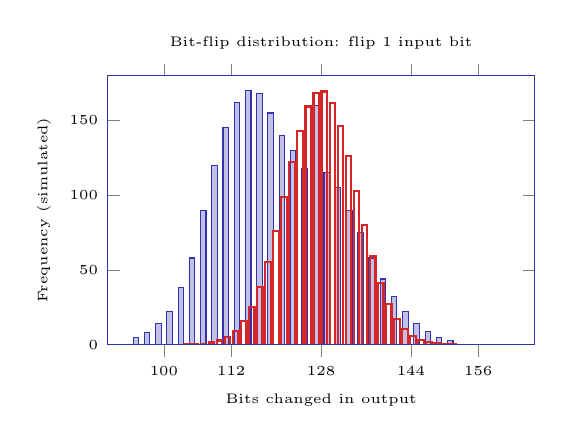
\begin{tikzpicture}
\begin{axis}[
  width=7cm, height=5cm,
  xlabel={Bits changed in output},
  ylabel={Frequency (simulated)},
  xmin=90,xmax=166,
  ymin=0,ymax=180,
  bar width=2pt,
  ybar,
  xtick={100,112,128,144,156},
  xticklabel style={font=\tiny},
  yticklabel style={font=\tiny},
  xlabel style={font=\tiny},
  ylabel style={font=\tiny},
  title style={font=\tiny},
  title={Bit-flip distribution: flip 1 input bit},
  fill=mllavender2,
  draw=mlpurple,
  area style,
]
\addplot[ybar,fill=mllavender2,draw=mlpurple] coordinates {
  (96,5)(98,8)(100,14)(102,22)(104,38)(106,58)(108,90)(110,120)(112,145)(114,162)
  (116,170)(118,168)(120,155)(122,140)(124,130)(126,118)(128,160)(130,115)(132,105)
  (134,90)(136,75)(138,58)(140,44)(142,32)(144,22)(146,14)(148,9)(150,5)(152,3)
};
\addplot[mlred,thick,domain=96:152,samples=40] {170*exp(-(x-127)^2/80)};
\end{axis}
\end{tikzpicture}
\column{0.46\textwidth}
\begin{block}{Avalanche Property}
Flipping 1 input bit flips $\approx n/2$ output bits:
\[E[\Delta\,\text{bits}] = \frac{n}{2} = 128\]
Variance $\approx n/4$; distribution $\approx \mathcal{N}(n/2,n/4)$.
\end{block}
\vspace{2mm}
\begin{block}{Implications for PoW}
\begin{itemize}\small
  \item Incrementing nonce produces completely different hash
  \item No shortcut: must try each nonce independently
  \item $P(\text{valid hash}) = T/2^{256}$ per attempt
  \item Mining is memoryless Bernoulli process
\end{itemize}
\end{block}
\end{columns}
\bottomnote{Strict avalanche criterion (SAC): flip any single input bit $\Rightarrow$ each output bit flips with prob 1/2}
\end{frame}

%--- FRAME 15: Hash Pointers ---
\begin{frame}{Hash Pointers: Building the Chain}
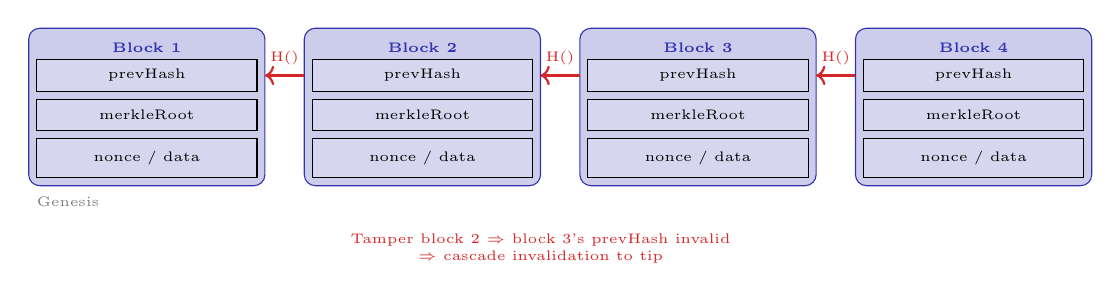
\begin{tikzpicture}[font=\small,node distance=0.3cm]
  \foreach \i/\x in {1/0, 2/3.5, 3/7.0, 4/10.5}{
    \draw[fill=mllavender3,draw=mlpurple,rounded corners] (\x,1.5) rectangle (\x+3.0,3.5);
    \node[font=\tiny\bfseries,mlpurple] at (\x+1.5,3.25) {Block \i};
    \draw[fill=mllavender4] (\x+0.1,2.7) rectangle (\x+2.9,3.1);
    \node[font=\tiny] at (\x+1.5,2.9) {prevHash};
    \draw[fill=mllavender4] (\x+0.1,2.2) rectangle (\x+2.9,2.6);
    \node[font=\tiny] at (\x+1.5,2.4) {merkleRoot};
    \draw[fill=mllavender4] (\x+0.1,1.6) rectangle (\x+2.9,2.1);
    \node[font=\tiny] at (\x+1.5,1.85) {nonce / data};
  }
  \draw[->,mlred,thick] (3.5,2.9) -- (3.0,2.9) node[midway,above,font=\tiny,mlred]{H()};
  \draw[->,mlred,thick] (7.0,2.9) -- (6.5,2.9) node[midway,above,font=\tiny,mlred]{H()};
  \draw[->,mlred,thick] (10.5,2.9) -- (10.0,2.9) node[midway,above,font=\tiny,mlred]{H()};
  \node[font=\tiny,mlgray] at (0.5,1.3) {Genesis};
  \node[font=\tiny,mlred,align=center] at (6.5,0.7) {Tamper block 2 $\Rightarrow$ block 3's prevHash invalid\\ $\Rightarrow$ cascade invalidation to tip};
\end{tikzpicture}
\vspace{2mm}
\begin{columns}
\column{0.5\textwidth}
\begin{block}{Tamper Detection}\small
If adversary modifies block $k$:
\begin{enumerate}
  \item Block $k$'s hash changes
  \item Block $k+1$'s prevHash no longer matches
  \item All subsequent blocks invalid
  \item Must re-mine from block $k$ onward
\end{enumerate}
\end{block}
\column{0.48\textwidth}
\begin{block}{Immutability Cost}
Cost to rewrite history from block $k$:
\[\text{Work} = \sum_{i=k}^{\text{tip}} D_i \cdot 2^{32}\;\text{hashes}\]
With current difficulty $D\approx 10^{13}$, rewriting 6 blocks requires $\approx 6\times 10^{13}\times 2^{32}$ hashes.
\end{block}
\end{columns}
\bottomnote{Hash pointers provide tamper-evidence; PoW makes tampering computationally infeasible}
\end{frame}

%--- FRAME 16: Birthday Paradox ---
\begin{frame}{Birthday Paradox \& Collision Security}
\begin{columns}
\column{0.52\textwidth}
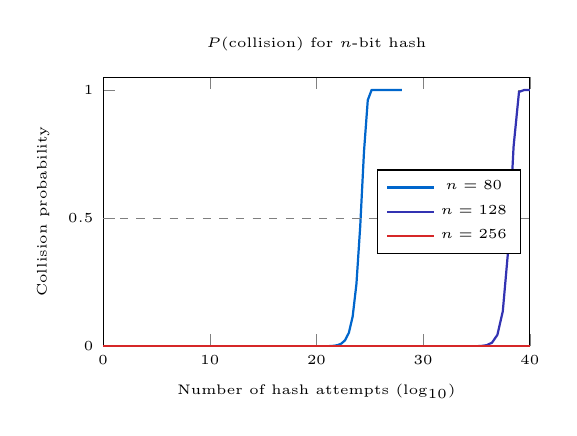
\begin{tikzpicture}
\begin{axis}[
  width=7cm, height=5cm,
  xlabel={Number of hash attempts ($\log_{10}$)},
  ylabel={Collision probability},
  xmin=0, xmax=40,
  ymin=0, ymax=1.05,
  xtick={0,10,20,30,40},
  xticklabel style={font=\tiny},
  yticklabel style={font=\tiny},
  xlabel style={font=\tiny},
  ylabel style={font=\tiny},
  title={$P(\text{collision})$ for $n$-bit hash},
  title style={font=\tiny},
  legend style={font=\tiny,at={(0.98,0.5)},anchor=east},
]
\addplot[mlblue,thick,domain=0:28,samples=80] {1-exp(-10^(x-24)/2)};
\addlegendentry{$n=80$}
\addplot[mlpurple,thick,domain=0:40,samples=80] {1-exp(-10^(x-38)/2)};
\addlegendentry{$n=128$}
\addplot[mlred,thick,domain=0:40,samples=80] {1-exp(-10^(x-77)/2)};
\addlegendentry{$n=256$}
\addplot[mlgray,dashed] coordinates {(0,0.5)(40,0.5)};
\node[font=\tiny,mlgray] at (35,0.55) {50\%};
\end{axis}
\end{tikzpicture}
\column{0.46\textwidth}
\begin{block}{Birthday Bound}
For $n$-bit hash, expect first collision after $\approx 2^{n/2}$ attempts:
\[P(\text{collision after } k) \approx 1-e^{-k^2/2^{n+1}}\]
At $k=2^{n/2}$: $P\approx 1-e^{-1/2}\approx 0.39$.
\end{block}
\vspace{2mm}
\begin{block}{SHA-256 Security}
\begin{itemize}\small
  \item Preimage: $2^{256}$ operations
  \item Collision: $2^{128}$ operations
  \item $2^{128} \approx 3.4\times10^{38}$: infeasible classically
  \item Quantum (Grover): $2^{64}$ -- still large
\end{itemize}
\end{block}
\end{columns}
\bottomnote{Birthday attack on 256-bit hash requires $2^{128}$ hashes; Bitcoin network does $\sim10^{20}$ hashes/year}
\end{frame}

%--- FRAME 17: Tamper Detection ---
\begin{frame}{Cascade Invalidation: Tamper Proof by Design}
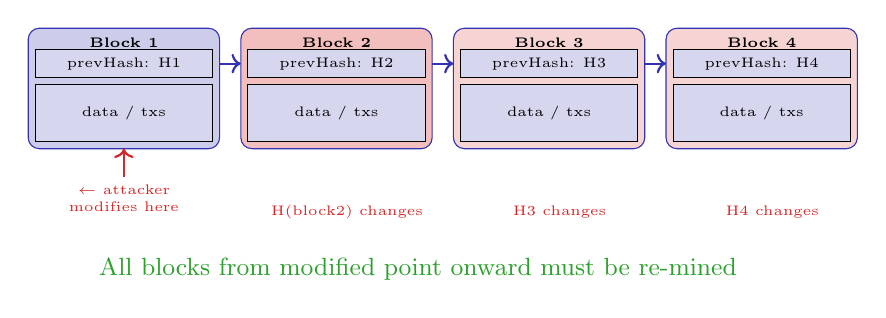
\begin{tikzpicture}[font=\tiny,scale=0.9]
  \foreach \i/\x/\col in {1/0/mllavender3, 2/3/mlred!30, 3/6/mlred!20, 4/9/mlred!20}{
    \draw[fill=\col,draw=mlpurple,rounded corners] (\x,1.5) rectangle (\x+2.7,3.2);
    \node[font=\tiny\bfseries] at (\x+1.35,3.0) {Block \i};
    \draw[fill=mllavender4] (\x+0.1,2.5) rectangle (\x+2.6,2.9);
    \node at (\x+1.35,2.7) {prevHash: H\i};
    \draw[fill=mllavender4] (\x+0.1,1.6) rectangle (\x+2.6,2.4);
    \node at (\x+1.35,2.0) {data / txs};
  }
  \draw[->,thick,mlpurple] (2.7,2.7)--(3.0,2.7);
  \draw[->,thick,mlpurple] (5.7,2.7)--(6.0,2.7);
  \draw[->,thick,mlpurple] (8.7,2.7)--(9.0,2.7);
  \node[mlred,font=\tiny,align=center] at (1.35,0.8) {$\leftarrow$ attacker\\modifies here};
  \draw[->,mlred,thick] (1.35,1.1)--(1.35,1.5);
  \node[mlred,font=\tiny] at (4.5,0.6) {H(block2) changes};
  \node[mlred,font=\tiny] at (7.5,0.6) {H3 changes};
  \node[mlred,font=\tiny] at (10.5,0.6) {H4 changes};
  \node[mlgreen,font=\small,align=center] at (5.5,-0.2) {All blocks from modified point onward must be re-mined};
\end{tikzpicture}
\vspace{3mm}
\begin{columns}
\column{0.48\textwidth}
\begin{block}{Re-mining Cost}\small
To rewrite from block $k$ to current height $N$:
\[\text{Expected hashes} = \sum_{i=k}^{N} D_i \times 2^{32}\]
$\approx (N-k)\times D \times 2^{32}$ if difficulty constant.
\end{block}
\column{0.48\textwidth}
\begin{block}{6-Confirmation Rule}\small
After 6 confirmations, probability honest chain extended faster than attacker chain (with $q<0.3$):
\[P(\text{success})<0.001\]
Merchants wait 6 blocks for high-value payments.
\end{block}
\end{columns}
\bottomnote{Immutability is probabilistic: each additional block exponentially increases rewrite cost}
\end{frame}

\section{Merkle Trees}

%--- FRAME 18: Binary Hash Tree ---
\begin{frame}{Merkle Tree: Binary Hash Tree}
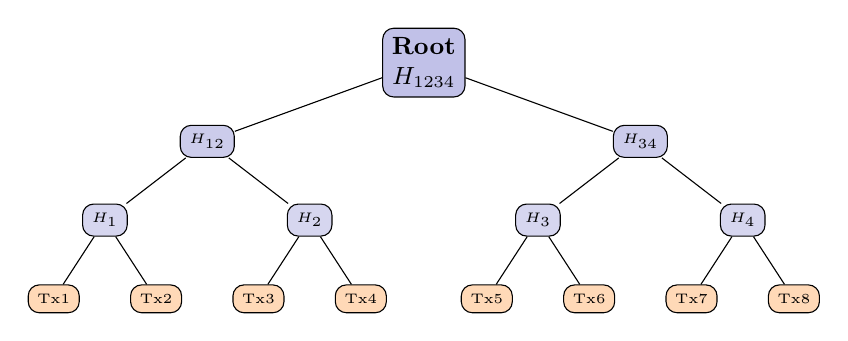
\begin{tikzpicture}[font=\tiny,level distance=1.0cm,
  level 1/.style={sibling distance=5.5cm},
  level 2/.style={sibling distance=2.6cm},
  level 3/.style={sibling distance=1.3cm}]
\node[draw,fill=mllavender2,rounded corners,font=\small\bfseries,align=center] {Root\\$H_{1234}$}
  child { node[draw,fill=mllavender3,rounded corners] {$H_{12}$}
    child { node[draw,fill=mllavender4,rounded corners] {$H_1$}
      child { node[draw,fill=mlorange!30,rounded corners] {Tx1} }
      child { node[draw,fill=mlorange!30,rounded corners] {Tx2} }
    }
    child { node[draw,fill=mllavender4,rounded corners] {$H_2$}
      child { node[draw,fill=mlorange!30,rounded corners] {Tx3} }
      child { node[draw,fill=mlorange!30,rounded corners] {Tx4} }
    }
  }
  child { node[draw,fill=mllavender3,rounded corners] {$H_{34}$}
    child { node[draw,fill=mllavender4,rounded corners] {$H_3$}
      child { node[draw,fill=mlorange!30,rounded corners] {Tx5} }
      child { node[draw,fill=mlorange!30,rounded corners] {Tx6} }
    }
    child { node[draw,fill=mllavender4,rounded corners] {$H_4$}
      child { node[draw,fill=mlorange!30,rounded corners] {Tx7} }
      child { node[draw,fill=mlorange!30,rounded corners] {Tx8} }
    }
  };
\end{tikzpicture}
\vspace{2mm}
\begin{block}{Construction Algorithm}
$H_i = \text{SHA256}^2(\text{Tx}_i)$;\quad $H_{ij}=\text{SHA256}^2(H_i\|H_j)$;\quad Root$=\text{SHA256}^2(H_{12}\|H_{34})$.
For odd count: last leaf duplicated. Root stored in block header.
\end{block}
\bottomnote{Merkle root: 32-byte commitment to all transactions; any tx change $\Rightarrow$ root changes}
\end{frame}

%--- FRAME 19: Merkle Proof SPV ---
\begin{frame}{Merkle Proof \& SPV Clients}
\begin{columns}
\column{0.5\textwidth}
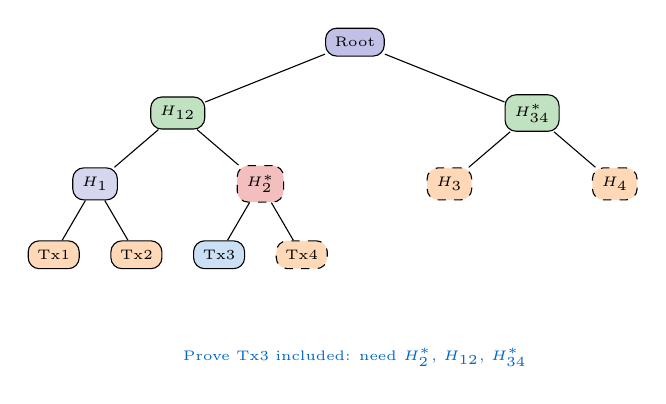
\begin{tikzpicture}[font=\tiny,level distance=0.9cm,
  level 1/.style={sibling distance=4.5cm},
  level 2/.style={sibling distance=2.1cm},
  level 3/.style={sibling distance=1.05cm}]
\node[draw,fill=mllavender2,rounded corners] {Root}
  child { node[draw,fill=mlgreen!30,rounded corners] {$H_{12}$}
    child { node[draw,fill=mllavender4,rounded corners] {$H_1$}
      child { node[draw,fill=mlorange!30,rounded corners] {Tx1} }
      child { node[draw,fill=mlorange!30,rounded corners] {Tx2} }
    }
    child { node[draw,fill=mlred!30,rounded corners,dashed] {$H_2^*$}
      child { node[draw,fill=mlblue!20,rounded corners] {Tx3\checkmark} }
      child { node[draw,fill=mlorange!30,rounded corners,dashed] {Tx4} }
    }
  }
  child { node[draw,fill=mlgreen!30,rounded corners] {$H_{34}^*$}
    child { node[draw,fill=mlorange!30,rounded corners,dashed] {$H_3$} }
    child { node[draw,fill=mlorange!30,rounded corners,dashed] {$H_4$} }
  };
\node[font=\tiny,mlblue] at (0,-4.0) {Prove Tx3 included: need $H_2^*$, $H_{12}$, $H_{34}^*$};
\end{tikzpicture}
\column{0.48\textwidth}
\begin{block}{Proof Size}
For $n$ transactions, proof requires $\lceil\log_2 n\rceil$ hashes:
\begin{center}
\begin{tabular}{lll}
\toprule
$n$ txs & Proof hashes & Size\\
\midrule
16 & 4 & 128 B\\
1,000 & 10 & 320 B\\
1M & 20 & 640 B\\
1B & 30 & 960 B\\
\bottomrule
\end{tabular}
\end{center}
\end{block}
\vspace{2mm}
\begin{block}{SPV Client}
\small Downloads headers only (80 B/block). Requests Merkle proof for specific tx. Verifies without full blockchain ($<$1 GB vs $>$500 GB).
\end{block}
\end{columns}
\bottomnote{SPV: Simplified Payment Verification (Bitcoin whitepaper, Section 8); enables lightweight wallets}
\end{frame}

%--- FRAME 20: Merkle Verification Algorithm ---
\begin{frame}[fragile]{Merkle Proof Verification}
\begin{columns}
\column{0.5\textwidth}
\begin{block}{Pseudocode}
\begin{lstlisting}
def verify_merkle_proof(tx, proof, root):
    """
    tx    : transaction bytes
    proof : list of (hash, side) pairs
            side in {'left', 'right'}
    root  : claimed Merkle root
    """
    current = sha256d(tx)
    for (sibling, side) in proof:
        if side == 'left':
            current = sha256d(sibling + current)
        else:
            current = sha256d(current + sibling)
    return current == root

# Example: prove Tx3 in 8-tx block
proof = [
    (H_Tx4, 'right'),   # H2 = H(Tx3||Tx4)
    (H_12,  'left'),    # H_1234 = H(H12||H34)
    (H_34,  'right'),
]
assert verify_merkle_proof(Tx3, proof, root)
\end{lstlisting}
\end{block}
\column{0.48\textwidth}
\begin{block}{Complexity Analysis}
\begin{tabular}{ll}
\toprule
Operation & Cost\\
\midrule
Build tree & $\mathcal{O}(n)$ hashes\\
Proof size & $\mathcal{O}(\log n)$ hashes\\
Verification & $\mathcal{O}(\log n)$ hashes\\
Storage (full) & $\mathcal{O}(n)$ hashes\\
\bottomrule
\end{tabular}
\end{block}
\vspace{2mm}
\begin{block}{Security}\small
An adversary cannot forge a valid proof for a transaction not in the tree (preimage resistance + collision resistance of SHA-256).
\end{block}
\vspace{2mm}
\begin{alertblock}{CVE Note}\small
Duplicate-leaf vulnerability: duplicate internal nodes can cause false inclusion proofs in some implementations.
\end{alertblock}
\end{columns}
\bottomnote{Bitcoin Core: merkle.cpp; OpenSSL used until 2015; now native SHA-256 implementation}
\end{frame}

%--- FRAME 21: Merkle Efficiency ---
\begin{frame}{Merkle Tree Efficiency}
\begin{columns}
\column{0.52\textwidth}
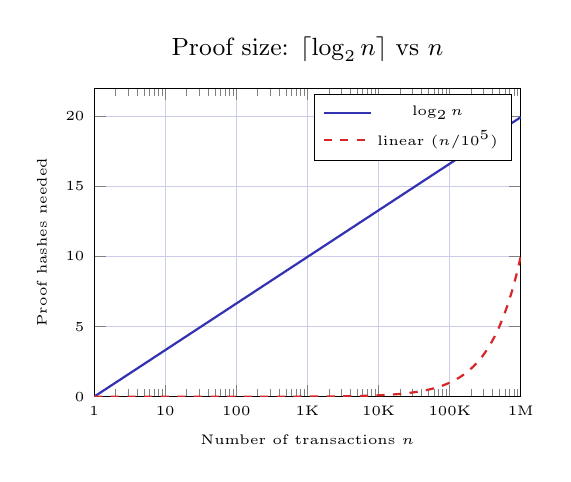
\begin{tikzpicture}
\begin{axis}[
  width=7cm, height=5.5cm,
  xlabel={Number of transactions $n$},
  ylabel={Proof hashes needed},
  xmin=1, xmax=1000000,
  ymin=0, ymax=22,
  xmode=log,
  xtick={1,10,100,1000,10000,100000,1000000},
  xticklabels={1,10,100,1K,10K,100K,1M},
  xticklabel style={font=\tiny},
  yticklabel style={font=\tiny},
  xlabel style={font=\tiny},
  ylabel style={font=\tiny},
  title={\small Proof size: $\lceil\log_2 n\rceil$ vs $n$},
  title style={font=\tiny},
  grid=major,
  grid style={mllavender3},
]
\addplot[mlpurple,thick,domain=1:1000000,samples=100] {ln(x)/ln(2)};
\addplot[mlred,dashed,thick,domain=1:1000000,samples=100] {x/100000};
\addlegendentry{\tiny $\log_2 n$}
\addlegendentry{\tiny linear ($n/10^5$)}
\end{axis}
\end{tikzpicture}
\column{0.46\textwidth}
\begin{block}{Why Logarithmic Matters}
\begin{itemize}\small
  \item 1 million transactions in block
  \item Linear proof: 1,000,000 hashes = 32 MB
  \item Merkle proof: 20 hashes = 640 bytes
  \item Speedup: $\times 50,000$
\end{itemize}
\end{block}
\vspace{2mm}
\begin{block}{Applications Beyond Bitcoin}
\begin{itemize}\small
  \item Git: content-addressed object store
  \item Certificate transparency logs
  \item IPFS / Filecoin storage proofs
  \item zk-SNARKs: Merkle membership proofs
  \item Ethereum state trie (Patricia Merkle)
\end{itemize}
\end{block}
\end{columns}
\bottomnote{Merkle trees: Ralph Merkle (1979); fundamental data structure for authenticated data}
\end{frame}

%--- FRAME 22: Patricia Merkle Tries ---
\begin{frame}{Patricia Merkle Trie (Ethereum)}
\begin{columns}
\column{0.5\textwidth}
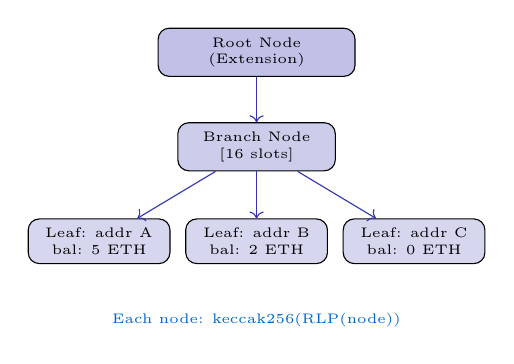
\begin{tikzpicture}[font=\tiny,node distance=0.5cm]
  \node[draw,fill=mllavender2,rounded corners,minimum width=2.5cm,align=center] (root) at (3,5.2) {Root Node\\(Extension)};
  \node[draw,fill=mllavender3,rounded corners,minimum width=2.0cm,align=center] (branch) at (3,4.0) {Branch Node\\{[16 slots]}};
  \node[draw,fill=mllavender4,rounded corners,minimum width=1.8cm,align=center] (leaf1) at (1.0,2.8) {Leaf: addr A\\bal: 5 ETH};
  \node[draw,fill=mllavender4,rounded corners,minimum width=1.8cm,align=center] (leaf2) at (3.0,2.8) {Leaf: addr B\\bal: 2 ETH};
  \node[draw,fill=mllavender4,rounded corners,minimum width=1.8cm,align=center] (leaf3) at (5.0,2.8) {Leaf: addr C\\bal: 0 ETH};
  \draw[->,mlpurple] (root)--(branch);
  \draw[->,mlpurple] (branch)--(leaf1);
  \draw[->,mlpurple] (branch)--(leaf2);
  \draw[->,mlpurple] (branch)--(leaf3);
  \node[font=\tiny,mlblue] at (3,1.8) {Each node: keccak256(RLP(node))};
\end{tikzpicture}
\column{0.48\textwidth}
\begin{block}{Three Node Types}
\begin{itemize}\small
  \item \textbf{Extension}: shared prefix compression
  \item \textbf{Branch}: 16-slot array (hex nibble)
  \item \textbf{Leaf}: terminal key-value pair
\end{itemize}
\end{block}
\vspace{2mm}
\begin{block}{Four Ethereum Tries}
\begin{tabular}{ll}
\toprule
Trie & Keys / Values\\
\midrule
State & address $\to$ account\\
Storage & slot $\to$ value (per contract)\\
Transaction & index $\to$ tx\\
Receipt & index $\to$ receipt\\
\bottomrule
\end{tabular}
\end{block}
\end{columns}
\bottomnote{Patricia Merkle Trie: combines Patricia trie (space efficiency) + Merkle (authentication)}
\end{frame}

\section{Proof of Work}

%--- FRAME 23: PoW Definition ---
\begin{frame}{Proof of Work: Mathematical Definition}
\begin{block}{Mining Condition}
\[\text{SHA256}^2(\underbrace{\text{version}\|\text{prevHash}\|\text{merkleRoot}\|\text{time}\|\text{bits}}_{\text{fixed for mining round}}\|\underbrace{\text{nonce}}_{\text{varied}}) < T\]
\end{block}
\vspace{2mm}
\begin{columns}
\column{0.5\textwidth}
\begin{block}{Target $T$ and Difficulty $D$}
\[T = \frac{T_{\max}}{D}, \qquad T_{\max} = 2^{224}\]
\[D \approx \frac{2^{224}}{T}\]
Current Bitcoin difficulty: $D \approx 8.7 \times 10^{13}$ (2024).\\[4pt]
Expected hashes per block:
\[E[\text{hashes}] = D \times 2^{32} \approx 3.7 \times 10^{23}\]
\end{block}
\column{0.48\textwidth}
\begin{block}{Probabilistic Interpretation}
Each hash attempt is an independent Bernoulli trial:
\[p = P(\text{valid hash}) = \frac{T}{2^{256}}\]
\[p \approx \frac{1}{D \times 2^{32}}\]
Number of attempts to find valid hash:
\[N \sim \text{Geometric}(p)\]
\[E[N] = \frac{1}{p} = D \times 2^{32}\]
\end{block}
\end{columns}
\bottomnote{PoW: computationally expensive to produce, trivially cheap to verify; asymmetric by design}
\end{frame}

%--- FRAME 24: Mining as Bernoulli Trials ---
\begin{frame}{Mining: Geometric Distribution}
\begin{columns}
\column{0.5\textwidth}
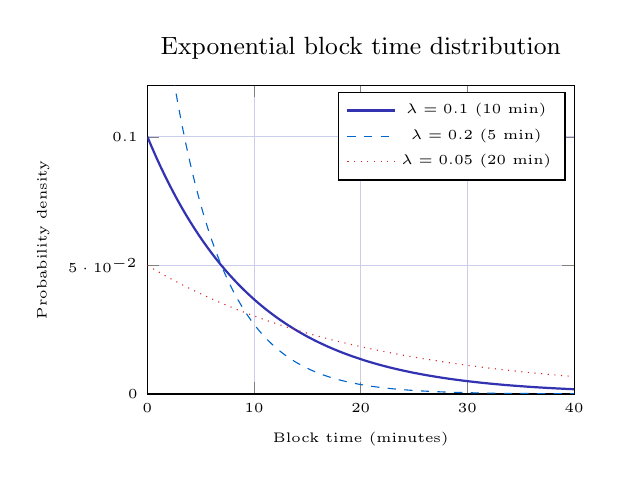
\begin{tikzpicture}
\begin{axis}[
  width=7cm, height=5.5cm,
  xlabel={Block time (minutes)},
  ylabel={Probability density},
  xmin=0, xmax=40,
  ymin=0, ymax=0.12,
  xticklabel style={font=\tiny},
  yticklabel style={font=\tiny},
  xlabel style={font=\tiny},
  ylabel style={font=\tiny},
  title={\small Exponential block time distribution},
  title style={font=\tiny},
  grid=major, grid style={mllavender3},
]
\addplot[mlpurple,thick,domain=0:40,samples=100] {0.1*exp(-0.1*x)};
\addlegendentry{\tiny $\lambda=0.1$ (10 min)}
\addplot[mlblue,dashed,domain=0:40,samples=100] {0.2*exp(-0.2*x)};
\addlegendentry{\tiny $\lambda=0.2$ (5 min)}
\addplot[mlred,dotted,domain=0:40,samples=100] {0.05*exp(-0.05*x)};
\addlegendentry{\tiny $\lambda=0.05$ (20 min)}
\end{axis}
\end{tikzpicture}
\column{0.48\textwidth}
\begin{block}{Memoryless Property}
Block inter-arrival time: $T \sim \text{Exp}(\lambda)$
\[P(T > t) = e^{-\lambda t}\]
\[\lambda = \frac{H}{D \times 2^{32}}\]
where $H$ = network hash rate.\\[4pt]
\textbf{Memoryless}: mining difficulty unchanged regardless of how long since last block.
\end{block}
\vspace{2mm}
\begin{block}{Multiple Miners}
With $n$ miners each with hash rate $h_i$:
\[P(\text{miner } i \text{ wins}) = \frac{h_i}{\sum_j h_j}\]
Mining is a race: proportional to hash power.
\end{block}
\end{columns}
\bottomnote{Bitcoin targets $\lambda=1/600$ (one block per 10 minutes); adjusted every 2016 blocks}
\end{frame}

%--- FRAME 25: Difficulty Adjustment ---
\begin{frame}{Difficulty Adjustment Algorithm}
\begin{columns}
\column{0.52\textwidth}
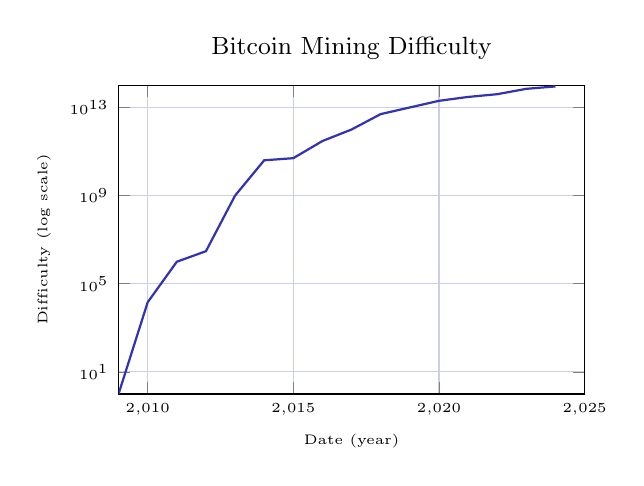
\begin{tikzpicture}
\begin{axis}[
  width=7.5cm, height=5.5cm,
  xlabel={Date (year)},
  ylabel={Difficulty (log scale)},
  xmin=2009, xmax=2025,
  ymode=log,
  ymin=1, ymax=1e14,
  xticklabel style={font=\tiny},
  yticklabel style={font=\tiny},
  xlabel style={font=\tiny},
  ylabel style={font=\tiny},
  title={\small Bitcoin Mining Difficulty},
  title style={font=\tiny},
  grid=major, grid style={mllavender3},
]
\addplot[mlpurple,thick] coordinates {
  (2009,1)(2010,14484)(2011,1e6)(2012,3e6)
  (2013,1e9)(2014,4e10)(2015,5e10)(2016,3e11)
  (2017,1e12)(2018,5e12)(2019,1e13)(2020,2e13)
  (2021,3e13)(2022,4e13)(2023,7e13)(2024,9e13)
};
\end{axis}
\end{tikzpicture}
\column{0.46\textwidth}
\begin{block}{Adjustment Formula}
Every 2016 blocks ($\approx$2 weeks):
\[D_{\text{new}} = D_{\text{old}} \times \frac{t_{\text{actual}}}{t_{\text{target}}}\]
where $t_{\text{target}} = 2016 \times 600 = 1{,}209{,}600$ s.\\[6pt]
\textbf{Clamped:} factor bounded by $[1/4, 4]$ to prevent extreme swings.
\end{block}
\vspace{2mm}
\begin{block}{Equilibrium Condition}
At steady state:
\[H = \frac{D \times 2^{32}}{600}\text{ H/s}\]
With $D=8.7\times10^{13}$: $H\approx 600$ EH/s.
\end{block}
\end{columns}
\bottomnote{Difficulty retarget: Bitcoin's self-regulating mechanism; hash rate tripled in 2023 yet blocks stay at 10 min}
\end{frame}

%--- FRAME 26: Mining Economics ---
\begin{frame}{Mining Economics}
\begin{columns}
\column{0.52\textwidth}
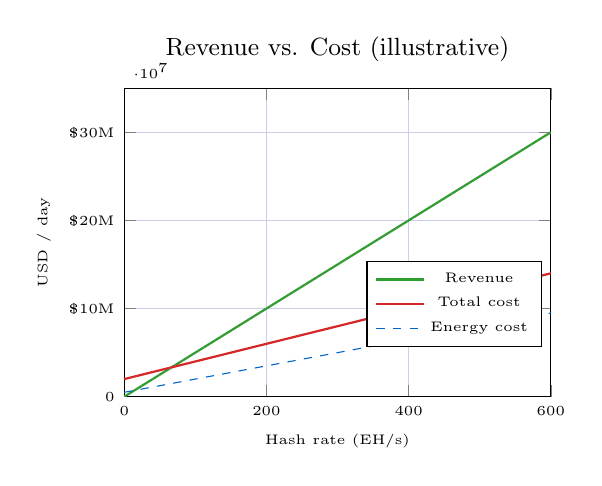
\begin{tikzpicture}
\begin{axis}[
  width=7cm, height=5.5cm,
  xlabel={Hash rate (EH/s)},
  ylabel={USD / day},
  xmin=0, xmax=600,
  ymin=0, ymax=35000000,
  xticklabel style={font=\tiny},
  yticklabel style={font=\tiny},
  xlabel style={font=\tiny},
  ylabel style={font=\tiny},
  ytick={0,10000000,20000000,30000000},
  yticklabels={0,\$10M,\$20M,\$30M},
  title={\small Revenue vs. Cost (illustrative)},
  title style={font=\tiny},
  legend style={font=\tiny,at={(0.98,0.3)},anchor=east},
  grid=major, grid style={mllavender3},
]
\addplot[mlgreen,thick,domain=0:600,samples=50] {50000*x};
\addlegendentry{Revenue}
\addplot[mlred,thick,domain=0:600,samples=50] {20000*x + 2000000};
\addlegendentry{Total cost}
\addplot[mlblue,dashed,domain=0:600,samples=50] {15000*x + 500000};
\addlegendentry{Energy cost}
\addplot[mlgray,dotted] coordinates {(0,0)(600,30000000)};
\end{axis}
\end{tikzpicture}
\column{0.46\textwidth}
\begin{block}{Revenue Formula}
\[\text{Rev}_i = \frac{h_i}{H}\left(R_{\text{sub}} + \sum_j f_j\right)\cdot P_{\text{BTC}}\]
where $h_i$ = miner hash rate, $H$ = total, $R_{\text{sub}}$ = block subsidy, $f_j$ = fees.
\end{block}
\vspace{2mm}
\begin{block}{Break-Even Condition}
\[\frac{h_i}{H}\cdot R\cdot P > c_{\text{elec}} \cdot h_i \cdot \frac{E}{\text{TH}}\]
$c_{\text{elec}}$: electricity cost (\$/kWh)\\
$E/\text{TH}$: energy efficiency (J/TH)\\
\textbf{Efficient miners survive; inefficient exit.}
\end{block}
\end{columns}
\bottomnote{Bitcoin mining: $\sim$\$20B revenue/year (2024); dominated by ASIC hardware (Antminer S21: 200 TH/s, 17.5 J/TH)}
\end{frame}

%--- FRAME 27: Hash Rate Distribution ---
\begin{frame}{Global Hash Rate Distribution (2024)}
\begin{columns}
\column{0.55\textwidth}
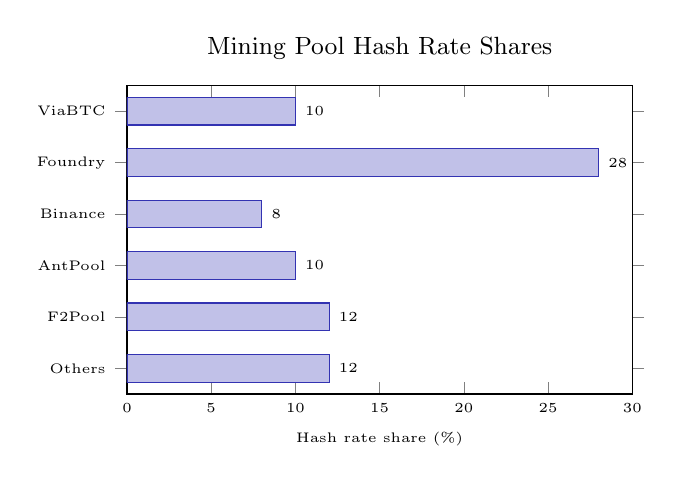
\begin{tikzpicture}
\begin{axis}[
  width=8cm, height=5.5cm,
  xbar,
  xlabel={Hash rate share (\%)},
  symbolic y coords={Others,F2Pool,AntPool,Binance,Foundry,ViaBTC},
  ytick=data,
  xmin=0, xmax=30,
  bar width=10pt,
  xticklabel style={font=\tiny},
  yticklabel style={font=\tiny},
  xlabel style={font=\tiny},
  nodes near coords,
  nodes near coords style={font=\tiny},
  title={\small Mining Pool Hash Rate Shares},
  title style={font=\tiny},
]
\addplot[fill=mllavender2,draw=mlpurple] coordinates {
  (12,Others)(12,F2Pool)(10,AntPool)(8,Binance)(28,Foundry)(10,ViaBTC)
};
\end{axis}
\end{tikzpicture}
\column{0.42\textwidth}
\begin{block}{Pool Economics}
\begin{itemize}\small
  \item Individual variance $\to$ pools reduce variance
  \item PPS (Pay Per Share): fixed rate per hash
  \item PPLNS: pay per last N shares
  \item Solo mining: $\sigma^2 \propto 1/h_i$
\end{itemize}
\end{block}
\vspace{2mm}
\begin{block}{Concentration Risk}
Top 3 pools often $>50\%$ of hash rate. Theoretical 51\% attack possible if colluding.\\[4pt]
\textbf{Nakamoto coefficient}: min pools needed to exceed 50\% = 2--3 (Bitcoin, 2024).
\end{block}
\end{columns}
\bottomnote{Mining centralization: geographic (60\% USA post-China ban) and pool-level concentration}
\end{frame}

%--- FRAME 28: Selfish Mining ---
\begin{frame}{Selfish Mining Attack}
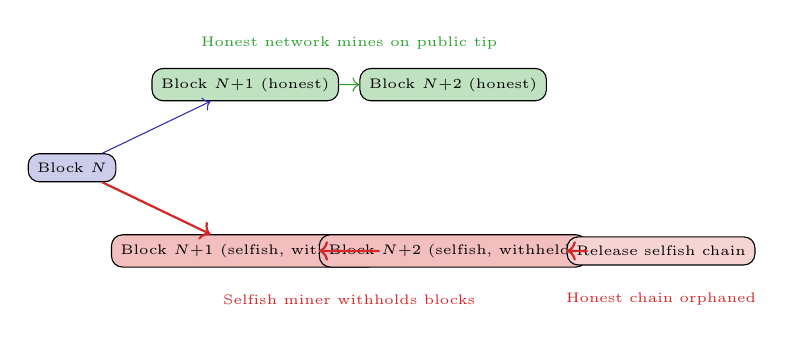
\begin{tikzpicture}[font=\tiny,scale=0.88]
  \node[draw,fill=mllavender3,rounded corners] (h0) at (0,2) {Block $N$};
  \node[draw,fill=mlgreen!30,rounded corners] (h1) at (2.5,3.2) {Block $N$+1 (honest)};
  \node[draw,fill=mlred!30,rounded corners] (s1) at (2.5,0.8) {Block $N$+1 (selfish, withheld)};
  \node[draw,fill=mlred!30,rounded corners] (s2) at (5.5,0.8) {Block $N$+2 (selfish, withheld)};
  \node[draw,fill=mlgreen!30,rounded corners] (h2) at (5.5,3.2) {Block $N$+2 (honest)};
  \node[draw,fill=mlred!20,rounded corners] (rel) at (8.5,0.8) {Release selfish chain};
  \draw[->,mlpurple] (h0)--(h1);
  \draw[->,mlred,thick] (h0)--(s1);
  \draw[->,mlred,thick] (s1)--(s2);
  \draw[->,mlgreen] (h1)--(h2);
  \draw[->,mlred,thick] (s2)--(rel);
  \node[font=\tiny,mlred] at (4,0.1) {Selfish miner withholds blocks};
  \node[font=\tiny,mlgreen] at (4,3.8) {Honest network mines on public tip};
  \node[font=\tiny,mlred] at (8.5,0.1) {Honest chain orphaned};
\end{tikzpicture}
\vspace{2mm}
\begin{columns}
\column{0.5\textwidth}
\begin{block}{Selfish Mining Threshold}
A pool with fraction $\alpha$ of hash rate can profitably selfish-mine when:
\[\alpha > \frac{1-\gamma}{3-2\gamma}\]
where $\gamma$ = fraction of honest miners who adopt the selfish chain when published simultaneously. Default: $\gamma=0$ gives $\alpha>1/3$.
\end{block}
\column{0.48\textwidth}
\begin{block}{Revenue Advantage}
Relative revenue of selfish miner:
\[R_{\text{selfish}} = \frac{\alpha(1-\alpha)^2(4\alpha+\gamma(1-2\alpha))-\alpha^3}{1-\alpha(1+(2-\alpha)\alpha)}\]
Exceeds $\alpha$ for $\alpha>1/3$ (worst case).
\end{block}
\end{columns}
\bottomnote{Eyal \& Sirer (2014): selfish mining profitable below 50\%; mitigated by FIFO propagation}
\end{frame}

%--- FRAME 29: Energy Consumption ---
\begin{frame}{Bitcoin Energy Consumption}
\begin{columns}
\column{0.55\textwidth}
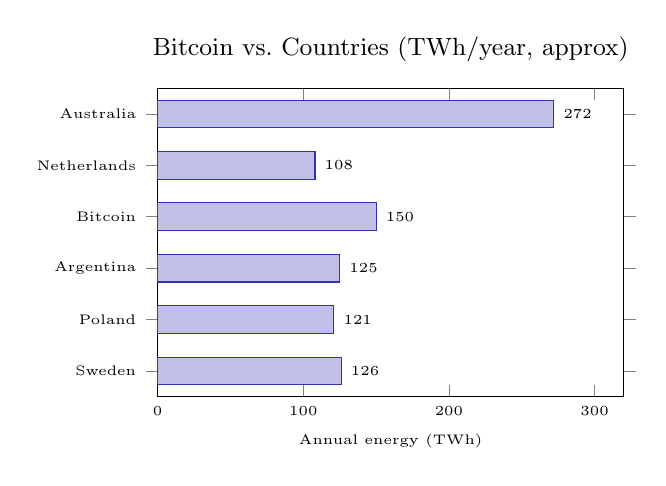
\begin{tikzpicture}
\begin{axis}[
  width=7.5cm, height=5.5cm,
  xbar,
  xlabel={Annual energy (TWh)},
  symbolic y coords={Sweden,Poland,Argentina,Bitcoin,Netherlands,Australia},
  ytick=data,
  xmin=0, xmax=320,
  bar width=10pt,
  xticklabel style={font=\tiny},
  yticklabel style={font=\tiny},
  xlabel style={font=\tiny},
  nodes near coords,
  nodes near coords style={font=\tiny},
  title={\small Bitcoin vs.\ Countries (TWh/year, approx)},
  title style={font=\tiny},
]
\addplot[fill=mllavender2,draw=mlpurple] coordinates {
  (126,Sweden)(121,Poland)(125,Argentina)(150,Bitcoin)(108,Netherlands)(272,Australia)
};
\end{axis}
\end{tikzpicture}
\column{0.42\textwidth}
\begin{block}{Energy Model}
\[\text{Energy} = H \cdot \frac{E_{\text{eff}}}{\text{TH/s}} \cdot \frac{1}{10^{12}}\text{ TW}\]
At $H=600$ EH/s, $E_{\text{eff}}=25$ J/TH:
\[\approx 600\times10^{18}\times25/(10^{12}) \approx 15\text{ GW}\]
$15\text{ GW} \times 8760\text{ h} \approx 131\text{ TWh/yr}$
\end{block}
\vspace{2mm}
\begin{block}{PoS Comparison}
Ethereum post-Merge: $\approx$0.01 TWh/yr (99.95\% reduction). Trade-off: different security model (economic vs. energy).
\end{block}
\end{columns}
\bottomnote{Bitcoin energy $\approx$ 0.4\% global electricity; \% of renewables disputed (est. 25--75\%)}
\end{frame}

\section{Proof of Stake}

%--- FRAME 30: PoS Definition ---
\begin{frame}{Proof of Stake: Mathematical Framework}
\begin{block}{Validator Selection Probability}
\[P(\text{validator } i \text{ selected}) = \frac{s_i}{\sum_{j=1}^{n} s_j}\]
where $s_i$ is the stake of validator $i$. Selection is proportional to economic stake.
\end{block}
\vspace{2mm}
\begin{columns}
\column{0.5\textwidth}
\begin{block}{Ethereum 2.0 Parameters}
\begin{tabular}{ll}
\toprule
\textbf{Parameter} & \textbf{Value}\\
\midrule
Min validator stake & 32 ETH\\
Max effective balance & 32 ETH\\
Epoch length & 32 slots\\
Slot duration & 12 seconds\\
Committee size & $\geq$128 validators\\
Finality & 2 epochs ($\approx$12.8 min)\\
\bottomrule
\end{tabular}
\end{block}
\column{0.48\textwidth}
\begin{block}{PoS Security Model}
Attack requires controlling $>1/3$ of staked ETH.\\[4pt]
Total staked: $\approx$ 30M ETH (2024).\\
Attack cost: $\frac{1}{3}\times 30\text{M ETH}\times\$3000 = \$30\text{B}$\\[4pt]
Additionally: slashing destroys attacker's stake, making attack economically self-destructive.
\end{block}
\end{columns}
\bottomnote{Ethereum PoS: $\sim$900,000 active validators (2024); $\approx$28\% of all ETH staked}
\end{frame}

%--- FRAME 31: Validator Lifecycle ---
\begin{frame}{Validator Lifecycle Automaton}
\begin{center}
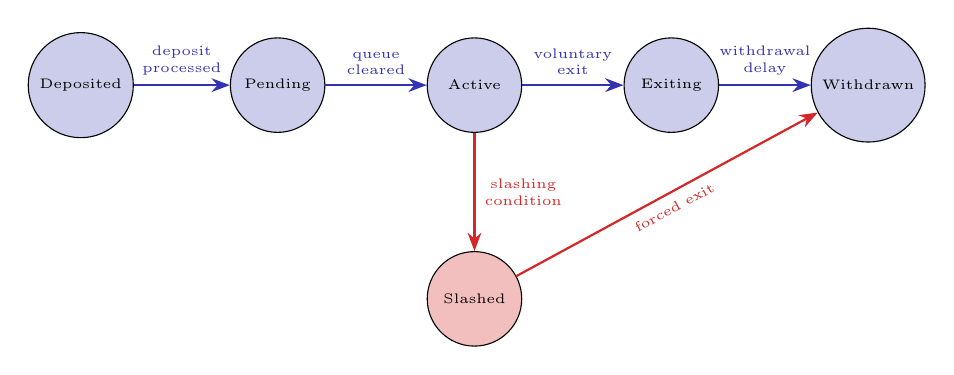
\begin{tikzpicture}[
  node distance=2.5cm,
  state/.style={draw,circle,fill=mllavender3,minimum size=1.2cm,font=\tiny,align=center},
  >=Stealth
]
  \node[state] (dep) {Deposited};
  \node[state,right of=dep] (pend) {Pending};
  \node[state,right of=pend] (act) {Active};
  \node[state,right of=act] (exit) {Exiting};
  \node[state,right of=exit] (with) {Withdrawn};
  \node[state,below=1.5cm of act,fill=mlred!30] (slash) {Slashed};
  \draw[->,mlpurple,thick] (dep)--(pend) node[midway,above,font=\tiny,align=center]{deposit\\processed};
  \draw[->,mlpurple,thick] (pend)--(act) node[midway,above,font=\tiny,align=center]{queue\\cleared};
  \draw[->,mlpurple,thick] (act)--(exit) node[midway,above,font=\tiny,align=center]{voluntary\\exit};
  \draw[->,mlpurple,thick] (exit)--(with) node[midway,above,font=\tiny,align=center]{withdrawal\\delay};
  \draw[->,mlred,thick] (act)--(slash) node[midway,right,font=\tiny,align=center]{slashing\\condition};
  \draw[->,mlred,thick] (slash)--(with) node[midway,below,font=\tiny,sloped]{forced exit};
\end{tikzpicture}
\end{center}
\vspace{2mm}
\begin{columns}
\column{0.48\textwidth}
\begin{block}{Queue Mechanics}\small
Entry and exit queues limit churn: max $\lfloor n_{\text{validators}}/65536\rfloor$ per epoch. At 900K validators: $\approx$13 entries/exits per epoch.
\end{block}
\column{0.48\textwidth}
\begin{block}{Withdrawal Delay}\small
After exit request: $\sim$256 epochs ($\approx$27 hours) before ETH unlocks. Prevents coordinated exit attacks.
\end{block}
\end{columns}
\bottomnote{Validator lifecycle: designed to maintain stability; sudden exits would threaten finality}
\end{frame}

%--- FRAME 32: Slashing Conditions ---
\begin{frame}{Slashing Conditions}
\begin{columns}
\column{0.5\textwidth}
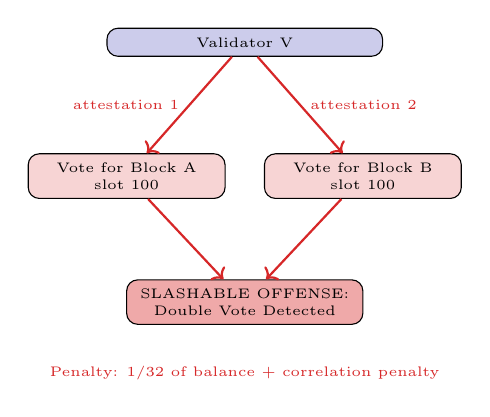
\begin{tikzpicture}[font=\tiny]
  \node[draw,fill=mllavender3,rounded corners,minimum width=3.5cm] (val) at (3,4.5) {Validator V};
  \node[draw,fill=mlred!20,rounded corners,minimum width=2.5cm,align=center] (b1) at (1.5,2.8) {Vote for Block A\\slot 100};
  \node[draw,fill=mlred!20,rounded corners,minimum width=2.5cm,align=center] (b2) at (4.5,2.8) {Vote for Block B\\slot 100};
  \draw[->,mlred,thick] (val)--(b1) node[midway,left,font=\tiny]{attestation 1};
  \draw[->,mlred,thick] (val)--(b2) node[midway,right,font=\tiny]{attestation 2};
  \node[draw,fill=mlred!40,rounded corners,minimum width=3cm,align=center] (slash) at (3,1.2) {SLASHABLE OFFENSE:\\Double Vote Detected};
  \draw[->,mlred,thick] (b1)--(slash);
  \draw[->,mlred,thick] (b2)--(slash);
  \node[font=\tiny,mlred] at (3,0.3) {Penalty: 1/32 of balance + correlation penalty};
\end{tikzpicture}
\column{0.48\textwidth}
\begin{block}{Two Slashing Offenses}
\textbf{1. Double voting (equivocation):}\\
Sign two different blocks at the same slot.
\[h_1 = h_2,\quad B_1 \neq B_2\]
\textbf{2. Surround voting:}\\
Vote with attestation that surrounds or is surrounded by a prior vote.
\[(e_1 < e_2 < e_3 < e_4) \wedge (e_1,e_4)\text{ surrounds }(e_2,e_3)\]
\end{block}
\vspace{2mm}
\begin{block}{Penalty Severity}
\small Correlation penalty: if many validators slashed simultaneously, penalty scales up to 100\% of stake (prevents coordinated attacks).
\end{block}
\end{columns}
\bottomnote{Slashing: game-theoretic deterrent; attacker loses stake while honest validators lose at most minor inactivity penalty}
\end{frame}

%--- FRAME 33: Nothing-at-Stake ---
\begin{frame}{Nothing-at-Stake Problem}
\begin{columns}
\column{0.5\textwidth}
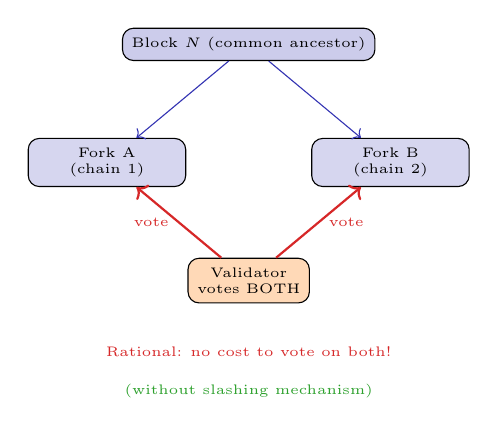
\begin{tikzpicture}[font=\tiny]
  \node[draw,fill=mllavender3,rounded corners] (parent) at (3,4.5) {Block $N$ (common ancestor)};
  \node[draw,fill=mllavender4,rounded corners,minimum width=2cm,align=center] (f1) at (1.2,3.0) {Fork A\\(chain 1)};
  \node[draw,fill=mllavender4,rounded corners,minimum width=2cm,align=center] (f2) at (4.8,3.0) {Fork B\\(chain 2)};
  \node[draw,fill=mlorange!30,rounded corners,minimum width=1.5cm,align=center] (val) at (3,1.5) {Validator\\votes BOTH};
  \draw[->,mlpurple] (parent)--(f1);
  \draw[->,mlpurple] (parent)--(f2);
  \draw[->,mlred,thick] (val)--(f1) node[midway,left,font=\tiny]{vote};
  \draw[->,mlred,thick] (val)--(f2) node[midway,right,font=\tiny]{vote};
  \node[font=\tiny,mlred] at (3,0.6) {Rational: no cost to vote on both!};
  \node[font=\tiny,mlgreen] at (3,0.1) {(without slashing mechanism)};
\end{tikzpicture}
\column{0.48\textwidth}
\begin{block}{The Problem}
In naive PoS: validator has no reason \emph{not} to vote on all forks. Cost = 0; expected reward = doubled.
\end{block}
\vspace{2mm}
\begin{block}{Solutions}
\begin{itemize}\small
  \item \textbf{Slashing}: double-voting destroys stake (economic deterrent)
  \item \textbf{Long-range attacks}: stake grinding mitigated by checkpointing
  \item \textbf{Finality gadgets} (Casper): make certain chain history permanent
  \item \textbf{Weak subjectivity}: new nodes accept recent finalized checkpoint
\end{itemize}
\end{block}
\end{columns}
\bottomnote{Nothing-at-stake solved by slashing; long-range attacks mitigated by weak subjectivity checkpoints}
\end{frame}

%--- FRAME 34: Casper FFG ---
\begin{frame}{Casper FFG: Finality Gadget}
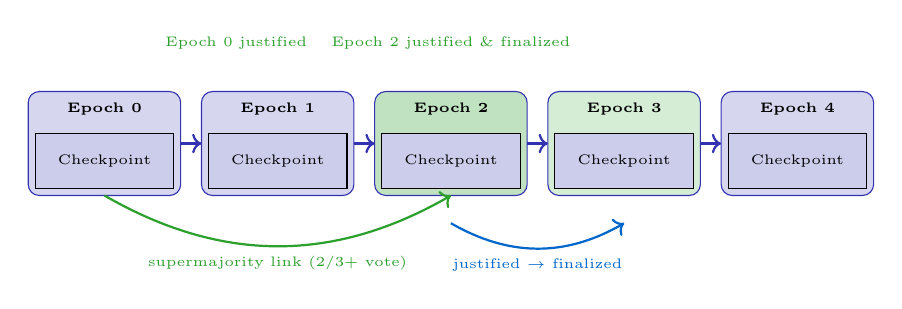
\begin{tikzpicture}[font=\small,scale=0.88]
  \foreach \i/\x/\col in {0/0/mllavender4, 1/2.5/mllavender4, 2/5.0/mlgreen!30, 3/7.5/mlgreen!20, 4/10.0/mllavender4}{
    \draw[fill=\col,draw=mlpurple,rounded corners] (\x,1.0) rectangle (\x+2.2,2.5);
    \node[font=\tiny\bfseries] at (\x+1.1,2.25) {Epoch \i};
    \draw[fill=mllavender3] (\x+0.1,1.1) rectangle (\x+2.1,1.9);
    \node[font=\tiny] at (\x+1.1,1.5) {Checkpoint};
  }
  \draw[->,mlpurple,thick] (2.2,1.75)--(2.5,1.75);
  \draw[->,mlpurple,thick] (4.7,1.75)--(5.0,1.75);
  \draw[->,mlpurple,thick] (7.2,1.75)--(7.5,1.75);
  \draw[->,mlpurple,thick] (9.7,1.75)--(10.0,1.75);
  \draw[mlgreen,thick,->] (1.1,1.0) to[bend right=30] node[below,font=\tiny]{supermajority link (2/3+ vote)} (6.1,1.0);
  \draw[mlblue,thick,->] (6.1,0.6) to[bend right=30] node[below,font=\tiny,mlblue]{justified $\to$ finalized} (8.6,0.6);
  \node[font=\tiny,mlgreen] at (3,3.2) {Epoch 0 justified};
  \node[font=\tiny,mlgreen] at (6.1,3.2) {Epoch 2 justified \& finalized};
\end{tikzpicture}
\vspace{2mm}
\begin{columns}
\column{0.5\textwidth}
\begin{block}{Justification \& Finalization}
\small A checkpoint $C$ is \textbf{justified} if $\geq2/3$ of validators vote for a supermajority link from a justified ancestor to $C$.\\[4pt]
$C$ is \textbf{finalized} if $C$ is justified and the next checkpoint is also justified via a direct link from $C$.
\end{block}
\column{0.48\textwidth}
\begin{block}{Safety Theorem}
Under Casper FFG: two conflicting checkpoints \emph{cannot both be finalized} unless $\geq1/3$ of validators are slashed.
\[\text{If }B_1\perp B_2\text{ both finalized}\Rightarrow\geq\frac{1}{3}\text{ stake slashed}\]
\end{block}
\end{columns}
\bottomnote{Casper FFG (Buterin \& Griffith, 2017): first formal finality gadget with accountable safety}
\end{frame}

%--- FRAME 35: Block Finality ---
\begin{frame}{Block Finality: Probabilistic vs.\ Deterministic}
\begin{columns}
\column{0.5\textwidth}
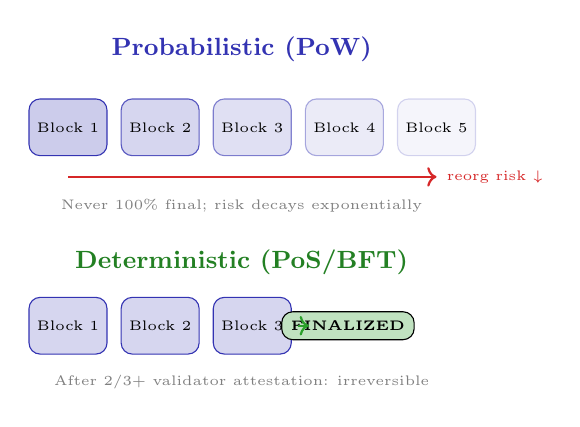
\begin{tikzpicture}[font=\tiny,scale=0.9]
  % Probabilistic finality (PoW)
  \node[font=\small\bfseries,mlpurple] at (3,5.5) {Probabilistic (PoW)};
  \foreach \i/\x/\op in {1/0/100, 2/1.3/80, 3/2.6/60, 4/3.9/40, 5/5.2/20}{
    \draw[fill=mllavender3,draw=mlpurple,rounded corners,opacity=\op/100] (\x,4.0) rectangle (\x+1.1,4.8);
    \node[font=\tiny] at (\x+0.55,4.4) {Block \i};
  }
  \draw[->,mlred,thick] (0.55,3.7) -- (5.75,3.7) node[right,font=\tiny]{reorg risk $\downarrow$};
  \node[font=\tiny,mlgray] at (3,3.3) {Never 100\% final; risk decays exponentially};
  % Deterministic finality (PoS)
  \node[font=\small\bfseries,mlgreen!80!black] at (3,2.5) {Deterministic (PoS/BFT)};
  \foreach \i/\x in {1/0, 2/1.3, 3/2.6}{
    \draw[fill=mllavender4,draw=mlpurple,rounded corners] (\x,1.2) rectangle (\x+1.1,2.0);
    \node[font=\tiny] at (\x+0.55,1.6) {Block \i};
  }
  \node[draw,fill=mlgreen!30,rounded corners,font=\tiny\bfseries] at (4.5,1.6) {FINALIZED};
  \draw[->,mlgreen,thick] (3.8,1.6) -- (3.95,1.6);
  \node[font=\tiny,mlgray] at (3,0.8) {After 2/3+ validator attestation: irreversible};
\end{tikzpicture}
\column{0.48\textwidth}
\begin{block}{Probabilistic Finality (Bitcoin)}
\begin{itemize}\small
  \item Confidence grows with each confirmation
  \item After $z$ blocks: $P(\text{reorg}) = (q/(1-q))^z$
  \item 6 confirmations: $\sim$60 min, $P < 0.001$
  \item Never mathematically ``final''
\end{itemize}
\end{block}
\vspace{2mm}
\begin{block}{Deterministic Finality (Ethereum)}
\begin{itemize}\small
  \item Casper FFG: finalized after 2 epochs ($\sim$13 min)
  \item Reversal requires slashing $\geq 1/3$ of total stake
  \item At 30M ETH staked: attack cost $>\$10$B
  \item Tendermint (Cosmos): single-slot finality ($\sim$6s)
\end{itemize}
\end{block}
\end{columns}
\bottomnote{Finality type determines confirmation time: PoW chains need minutes; BFT chains can finalize in seconds}
\end{frame}

%--- FRAME 36: Staking Economics ---
\begin{frame}{Staking Economics: Yield Curve}
\begin{columns}
\column{0.55\textwidth}
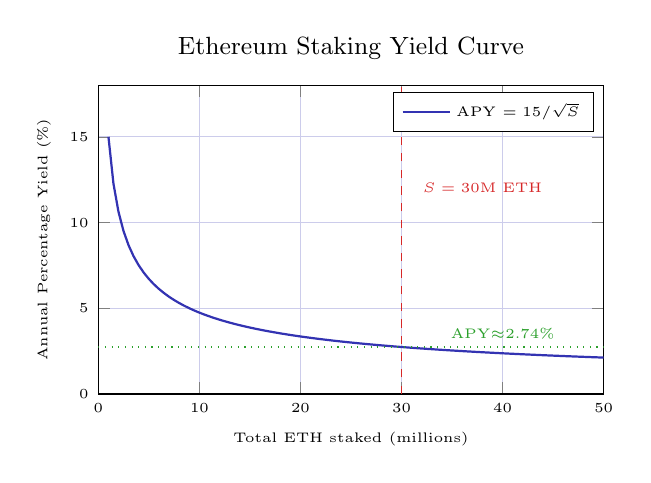
\begin{tikzpicture}
\begin{axis}[
  width=8cm, height=5.5cm,
  xlabel={Total ETH staked (millions)},
  ylabel={Annual Percentage Yield (\%)},
  xmin=0, xmax=50,
  ymin=0, ymax=18,
  xticklabel style={font=\tiny},
  yticklabel style={font=\tiny},
  xlabel style={font=\tiny},
  ylabel style={font=\tiny},
  title={\small Ethereum Staking Yield Curve},
  title style={font=\tiny},
  grid=major, grid style={mllavender3},
]
\addplot[mlpurple,thick,domain=1:50,samples=100] {15/sqrt(x)};
\addlegendentry{\tiny APY $= 15/\sqrt{S}$}
\addplot[mlred,dashed] coordinates {(30,0)(30,18)};
\addplot[mlgreen,dotted] coordinates {(0,2.74)(50,2.74)};
\node[font=\tiny,mlred] at (38,12) {$S=30$M ETH};
\node[font=\tiny,mlgreen] at (40,3.5) {APY$\approx$2.74\%};
\end{axis}
\end{tikzpicture}
\column{0.42\textwidth}
\begin{block}{Issuance Model}
Base reward per validator:
\[r = \frac{B_{\text{eff}} \times c}{\sqrt{\sum s_i}}\]
where $c$ is the base reward factor (64 in Ethereum), $B_{\text{eff}}$ = effective balance.\\[4pt]
Total issuance $\propto \sqrt{N_{\text{validators}}}$, but per-validator yield $\propto 1/\sqrt{N}$.
\end{block}
\vspace{2mm}
\begin{block}{Nash Equilibrium}
Staking equilibrium where marginal validator is indifferent between staking and alternatives. Current: $\sim$3--4\% APY.
\end{block}
\end{columns}
\bottomnote{Ethereum issuance: $\approx$600K ETH/year at 30M staked; deflationary post-EIP-1559 if burn $>$ issuance}
\end{frame}

%--- FRAME 36: PoW vs PoS Comparison ---
\begin{frame}{Proof of Work vs.\ Proof of Stake}
\begin{center}
\begin{tabular}{lll}
\toprule
\textbf{Property} & \textbf{Proof of Work} & \textbf{Proof of Stake}\\
\midrule
Security resource & Computation (hash rate) & Capital (staked tokens)\\
Attack cost & $>50\%$ hash rate & $>33\%$ staked value\\
Energy use & $\sim$130 TWh/yr (BTC) & $\sim$0.01 TWh/yr (ETH)\\
Finality & Probabilistic & Deterministic (Casper)\\
Hardware req. & ASIC / GPU & Standard computer\\
Centralization & Mining pools (geographic) & Stake concentration\\
Bootstrapping & CPU mining egalitarian & Rich-get-richer tendency\\
Reorg defense & Accumulated PoW & Slashing mechanism\\
Quantum risk & Moderate (Grover $\times2$) & ECDSA key exposure\\
Proven security & 15+ years (BTC) & 2+ years (ETH)\\
\bottomrule
\end{tabular}
\end{center}
\vspace{2mm}
\begin{columns}
\column{0.48\textwidth}
\begin{alertblock}{PoW Advantage}
\small Longest-chain rule is simple; security doesn't depend on protocol complexity; no slashing; no stake nothing-at-stake.
\end{alertblock}
\column{0.48\textwidth}
\begin{alertblock}{PoS Advantage}
\small Orders of magnitude less energy; fast finality; no ASIC arms race; stake as bond enables slashing deterrent.
\end{alertblock}
\end{columns}
\bottomnote{No consensus on ``better'': PoW = energy security model; PoS = economic security model}
\end{frame}

\section{Network}

%--- FRAME 37: P2P Topology ---
\begin{frame}{P2P Network Topology \& Gossip Propagation}
\begin{columns}
\column{0.5\textwidth}
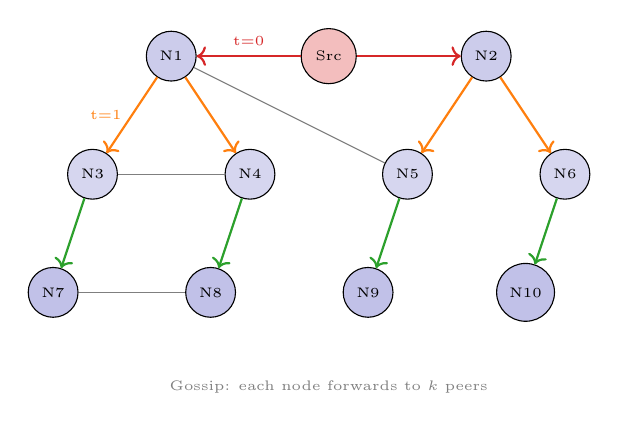
\begin{tikzpicture}[font=\tiny]
  \node[draw,circle,fill=mlred!30,minimum size=0.7cm] (src) at (4,4) {Src};
  \node[draw,circle,fill=mllavender3,minimum size=0.6cm] (n1) at (2,4) {N1};
  \node[draw,circle,fill=mllavender3,minimum size=0.6cm] (n2) at (6,4) {N2};
  \node[draw,circle,fill=mllavender4,minimum size=0.6cm] (n3) at (1,2.5) {N3};
  \node[draw,circle,fill=mllavender4,minimum size=0.6cm] (n4) at (3,2.5) {N4};
  \node[draw,circle,fill=mllavender4,minimum size=0.6cm] (n5) at (5,2.5) {N5};
  \node[draw,circle,fill=mllavender4,minimum size=0.6cm] (n6) at (7,2.5) {N6};
  \node[draw,circle,fill=mllavender2,minimum size=0.6cm] (n7) at (0.5,1) {N7};
  \node[draw,circle,fill=mllavender2,minimum size=0.6cm] (n8) at (2.5,1) {N8};
  \node[draw,circle,fill=mllavender2,minimum size=0.6cm] (n9) at (4.5,1) {N9};
  \node[draw,circle,fill=mllavender2,minimum size=0.6cm] (n10) at (6.5,1) {N10};
  \draw[->,mlred,thick] (src)--(n1) node[midway,above,font=\tiny]{t=0};
  \draw[->,mlred,thick] (src)--(n2);
  \draw[->,mlorange,thick] (n1)--(n3) node[midway,left,font=\tiny]{t=1};
  \draw[->,mlorange,thick] (n1)--(n4);
  \draw[->,mlorange,thick] (n2)--(n5);
  \draw[->,mlorange,thick] (n2)--(n6);
  \draw[->,mlgreen,thick] (n3)--(n7);
  \draw[->,mlgreen,thick] (n4)--(n8);
  \draw[->,mlgreen,thick] (n5)--(n9);
  \draw[->,mlgreen,thick] (n6)--(n10);
  \draw[mlgray] (n1)--(n5); \draw[mlgray] (n3)--(n4); \draw[mlgray] (n7)--(n8);
  \node[font=\tiny,mlgray,align=left] at (4,-0.2) {Gossip: each node forwards to $k$ peers};
\end{tikzpicture}
\column{0.48\textwidth}
\begin{block}{Gossip Protocol}
Each node maintains $\sim$8--125 peer connections. New block/tx: node relays to all peers except sender (``flooding'').\\[4pt]
Propagation time with $k$ connections per node:
\[t_{\text{prop}} \approx \frac{\log N}{\log k} \cdot t_{\text{hop}}\]
For $N=10{,}000$ nodes, $k=8$, $t_{\text{hop}}=100$ms: $t\approx 1.3$ s.
\end{block}
\vspace{2mm}
\begin{block}{Compact Block Relay}
Bitcoin: send header + short tx IDs; receiver reconstructs from mempool. Reduces bandwidth by $\sim$98\%.
\end{block}
\end{columns}
\bottomnote{Bitcoin P2P: $\sim$15,000 reachable full nodes; Ethereum: $\sim$7,000 nodes (2024)}
\end{frame}

%--- FRAME 38: Block Propagation ---
\begin{frame}{Block Propagation Time Distribution}
\begin{columns}
\column{0.55\textwidth}
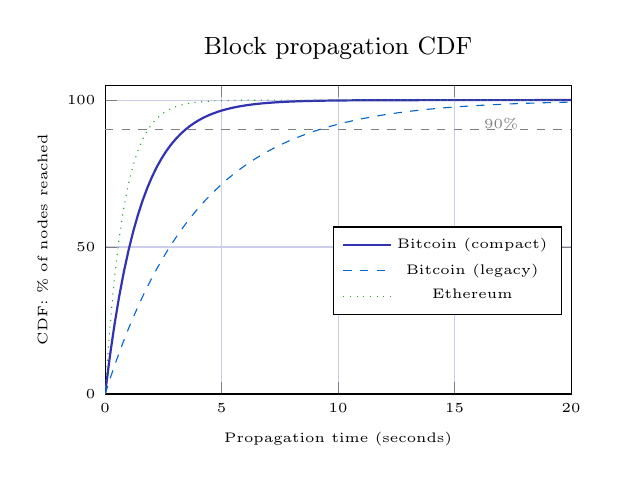
\begin{tikzpicture}
\begin{axis}[
  width=7.5cm, height=5.5cm,
  xlabel={Propagation time (seconds)},
  ylabel={CDF: \% of nodes reached},
  xmin=0, xmax=20,
  ymin=0, ymax=105,
  xticklabel style={font=\tiny},
  yticklabel style={font=\tiny},
  xlabel style={font=\tiny},
  ylabel style={font=\tiny},
  title={\small Block propagation CDF},
  title style={font=\tiny},
  legend style={font=\tiny,at={(0.98,0.4)},anchor=east},
  grid=major, grid style={mllavender3},
]
\addplot[mlpurple,thick,domain=0:20,samples=100] {100*(1-exp(-x/1.5))};
\addlegendentry{Bitcoin (compact)}
\addplot[mlblue,dashed,domain=0:20,samples=100] {100*(1-exp(-x/4.0))};
\addlegendentry{Bitcoin (legacy)}
\addplot[mlgreen,dotted,domain=0:20,samples=100] {100*(1-exp(-x/0.8))};
\addlegendentry{Ethereum}
\addplot[mlgray,dashed] coordinates {(0,90)(20,90)};
\node[font=\tiny,mlgray] at (17,92) {90\%};
\end{axis}
\end{tikzpicture}
\column{0.43\textwidth}
\begin{block}{Stale Block Rate}
Probability block becomes stale (orphaned):
\[\rho \approx 1 - e^{-\lambda t_{\text{prop}}}\]
For $t_{\text{prop}}=2$s, $\lambda=1/600$: $\rho\approx 0.33\%$\\[4pt]
\textbf{GHOST protocol} (Ethereum pre-merge): include ``uncle'' blocks to reduce waste.
\end{block}
\vspace{2mm}
\begin{block}{FIBRE Network}
Fast Internet Bitcoin Relay Engine: dedicated relay network reduces median propagation to $<$100ms for mining pools.
\end{block}
\end{columns}
\bottomnote{Slow propagation $\Rightarrow$ higher orphan rate $\Rightarrow$ large miners advantaged (pool centralization pressure)}
\end{frame}

%--- FRAME 39: Fork Resolution ---
\begin{frame}{Fork Types \& Resolution}
\begin{columns}
\column{0.5\textwidth}
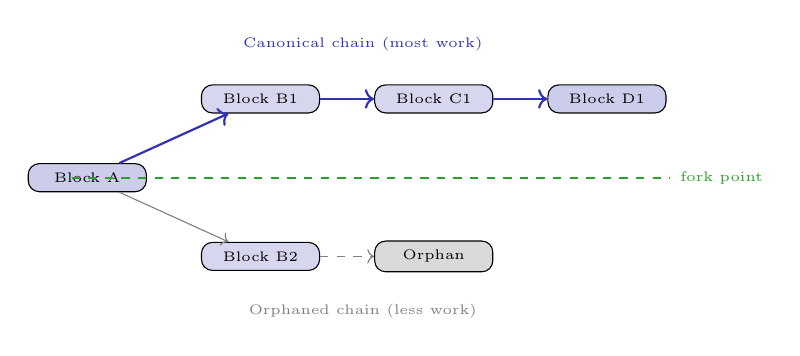
\begin{tikzpicture}[font=\tiny]
  \node[draw,fill=mllavender3,rounded corners,minimum width=1.5cm] (a) at (0,3) {Block A};
  \node[draw,fill=mllavender4,rounded corners,minimum width=1.5cm] (b1) at (2.2,4) {Block B1};
  \node[draw,fill=mllavender4,rounded corners,minimum width=1.5cm] (b2) at (2.2,2) {Block B2};
  \node[draw,fill=mllavender4,rounded corners,minimum width=1.5cm] (c1) at (4.4,4) {Block C1};
  \node[draw,fill=mlgray!30,rounded corners,minimum width=1.5cm] (c2) at (4.4,2) {Orphan};
  \node[draw,fill=mllavender3,rounded corners,minimum width=1.5cm] (d1) at (6.6,4) {Block D1};
  \draw[->,mlpurple,thick] (a)--(b1);
  \draw[->,mlgray] (a)--(b2);
  \draw[->,mlpurple,thick] (b1)--(c1);
  \draw[->,mlgray,dashed] (b2)--(c2);
  \draw[->,mlpurple,thick] (c1)--(d1);
  \node[font=\tiny,mlpurple] at (3.5,4.7) {Canonical chain (most work)};
  \node[font=\tiny,mlgray] at (3.5,1.3) {Orphaned chain (less work)};
  \draw[mlgreen,thick,dashed] (-0.2,3.0) -- (7.4,3.0) node[right,font=\tiny,mlgreen]{fork point};
\end{tikzpicture}
\column{0.48\textwidth}
\begin{block}{Nakamoto Longest Chain Rule}
\small When two valid chains exist, nodes always extend the chain with most accumulated proof-of-work (not longest by block count).\\[4pt]
\[\text{canonical} = \arg\max_{\text{chain}} \sum_{\text{blocks}} D_i\]
\end{block}
\vspace{2mm}
\begin{block}{Fork Types}
\begin{itemize}\small
  \item \textbf{Accidental}: natural propagation delay; resolved in 1--2 blocks
  \item \textbf{Soft fork}: tightens rules (backward compatible)
  \item \textbf{Hard fork}: loosens or changes rules (not backward compatible)
  \item \textbf{Contentious hard fork}: chain split (e.g., BCH, ETC)
\end{itemize}
\end{block}
\end{columns}
\bottomnote{Orphan rate: $\sim$0.3\% Bitcoin; Ethereum had $\sim$5\% uncle rate pre-merge (12s blocks)}
\end{frame}

%--- FRAME 40: Nakamoto Coefficient ---
\begin{frame}{Nakamoto Coefficient: Measuring Decentralization}
\begin{columns}
\column{0.55\textwidth}
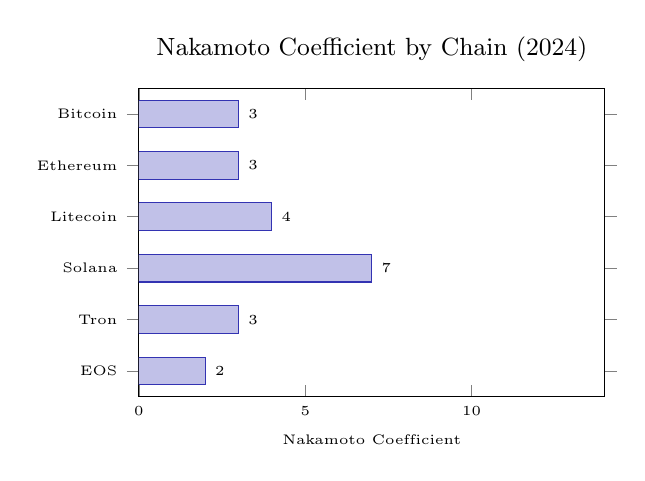
\begin{tikzpicture}
\begin{axis}[
  width=7.5cm, height=5.5cm,
  xbar,
  xlabel={Nakamoto Coefficient},
  symbolic y coords={EOS,Tron,Solana,Litecoin,Ethereum,Bitcoin},
  ytick=data,
  xmin=0, xmax=14,
  bar width=10pt,
  xticklabel style={font=\tiny},
  yticklabel style={font=\tiny},
  xlabel style={font=\tiny},
  nodes near coords,
  nodes near coords style={font=\tiny},
  title={\small Nakamoto Coefficient by Chain (2024)},
  title style={font=\tiny},
]
\addplot[fill=mllavender2,draw=mlpurple] coordinates {
  (2,EOS)(3,Tron)(7,Solana)(4,Litecoin)(3,Ethereum)(3,Bitcoin)
};
\end{axis}
\end{tikzpicture}
\column{0.43\textwidth}
\begin{block}{Definition}
\textbf{Nakamoto coefficient} $\mathcal{N}$: minimum number of entities that must collude to compromise consensus.
\[\mathcal{N} = \min k:\;\sum_{i=1}^{k} s_i > \frac{1}{2}\sum_{i=1}^{n} s_i\]
Higher $\mathcal{N}$ = more decentralized.
\end{block}
\vspace{2mm}
\begin{block}{Dimensions Measured}
\begin{itemize}\small
  \item Mining pools / validator sets
  \item Exchange custody
  \item Client software diversity
  \item Geography of nodes
  \item Developer concentration
\end{itemize}
\end{block}
\end{columns}
\bottomnote{Nakamoto coefficient: single-number proxy for decentralization; true security requires multidimensional analysis}
\end{frame}

%--- FRAME 41: Decentralization Metrics ---
\begin{frame}{Quantifying Decentralization}
\begin{columns}
\column{0.5\textwidth}
\begin{block}{Gini Coefficient}
Measures stake/hash rate inequality:
\[G = \frac{\sum_{i=1}^n\sum_{j=1}^n |s_i-s_j|}{2n\sum_{i=1}^n s_i}\]
$G=0$: perfect equality; $G=1$: one entity holds all.\\[4pt]
Bitcoin mining pools: $G\approx 0.7$\\
Ethereum validators: $G\approx 0.6$
\end{block}
\vspace{2mm}
\begin{block}{Shannon Entropy}
\[H = -\sum_{i=1}^n p_i \log_2 p_i\]
where $p_i = s_i / \sum_j s_j$.\\
Max entropy: $\log_2 n$ (all equal shares).
\end{block}
\column{0.48\textwidth}
\begin{block}{Herfindahl--Hirschman Index}
\[\text{HHI} = \sum_{i=1}^n \left(\frac{s_i}{\sum_j s_j}\right)^2 \times 10{,}000\]
$\text{HHI} < 1500$: competitive market.\\
$\text{HHI} > 2500$: highly concentrated.\\[6pt]
\textbf{Example}: 3 pools with 33\% each:\\
$\text{HHI} = 3\times(33)^2/100 = 3267$ (concentrated)
\end{block}
\vspace{2mm}
\begin{alertblock}{Limitation}
\small All metrics capture a single dimension. Real decentralization requires: geographic, client, ownership, and governance analysis.
\end{alertblock}
\end{columns}
\bottomnote{Decentralization is multidimensional; no single metric captures all aspects of blockchain security}
\end{frame}

%--- FRAME 43: Blockchain Governance Models ---
\begin{frame}{Blockchain Governance Models}
\begin{center}
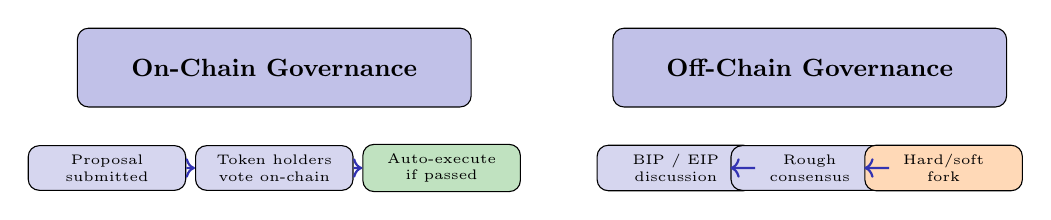
\begin{tikzpicture}[font=\small,scale=0.85]
  % On-chain governance
  \node[draw,fill=mllavender2,rounded corners,minimum width=5cm,minimum height=1.0cm,align=center] (onchain) at (3.5,5.0) {\textbf{On-Chain Governance}};
  \node[draw,fill=mllavender4,rounded corners,minimum width=2cm,font=\tiny,align=center] (prop) at (1,3.5) {Proposal\\submitted};
  \node[draw,fill=mllavender4,rounded corners,minimum width=2cm,font=\tiny,align=center] (vote) at (3.5,3.5) {Token holders\\vote on-chain};
  \node[draw,fill=mlgreen!30,rounded corners,minimum width=2cm,font=\tiny,align=center] (exec) at (6,3.5) {Auto-execute\\if passed};
  \draw[->,mlpurple,thick] (prop)--(vote);
  \draw[->,mlpurple,thick] (vote)--(exec);
  % Off-chain governance
  \node[draw,fill=mllavender2,rounded corners,minimum width=5cm,minimum height=1.0cm,align=center] (offchain) at (11.5,5.0) {\textbf{Off-Chain Governance}};
  \node[draw,fill=mllavender4,rounded corners,minimum width=2cm,font=\tiny,align=center] (bip) at (9.5,3.5) {BIP / EIP\\discussion};
  \node[draw,fill=mllavender4,rounded corners,minimum width=2cm,font=\tiny,align=center] (rough) at (11.5,3.5) {Rough\\consensus};
  \node[draw,fill=mlorange!30,rounded corners,minimum width=2cm,font=\tiny,align=center] (fork) at (13.5,3.5) {Hard/soft\\fork};
  \draw[->,mlpurple,thick] (bip)--(rough);
  \draw[->,mlpurple,thick] (rough)--(fork);
\end{tikzpicture}
\end{center}
\vspace{2mm}
\begin{columns}
\column{0.48\textwidth}
\begin{block}{On-Chain (Tezos, Polkadot)}
\begin{itemize}\small
  \item Protocol upgrades via token voting
  \item Automatic enactment after threshold
  \item DAOs: Decentralized Autonomous Organizations
  \item Risk: plutocracy (rich dominate votes)
\end{itemize}
\end{block}
\column{0.48\textwidth}
\begin{block}{Off-Chain (Bitcoin, Ethereum)}
\begin{itemize}\small
  \item BIPs/EIPs: formal improvement proposals
  \item Core devs, miners, users signal support
  \item Contentious changes $\to$ hard fork (e.g., BCH 2017)
  \item Slower but more conservative; ``code is not law''
\end{itemize}
\end{block}
\end{columns}
\bottomnote{Governance determines how blockchains evolve; no perfect model -- trade-off between speed and decentralization}
\end{frame}

%--- FRAME 44: Full Nodes vs Light Clients ---
\begin{frame}{Node Types: Full Nodes vs.\ Light Clients}
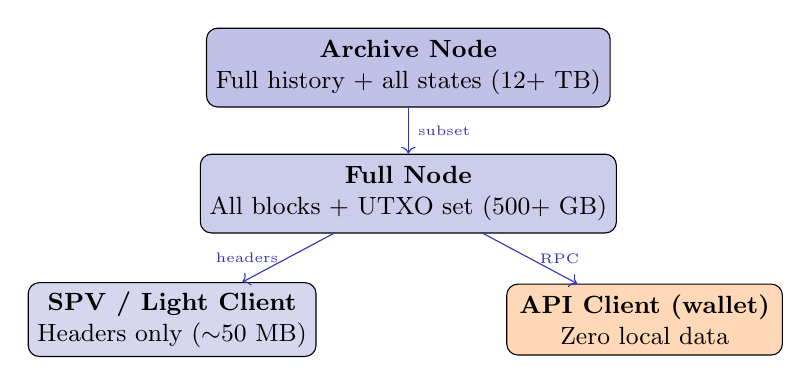
\begin{tikzpicture}[font=\small]
  \node[draw,fill=mllavender2,rounded corners,minimum width=4cm,minimum height=1.0cm,align=center] (arch) at (5,4.8) {\textbf{Archive Node}\\Full history + all states (12+ TB)};
  \node[draw,fill=mllavender3,rounded corners,minimum width=4cm,minimum height=1.0cm,align=center] (full) at (5,3.2) {\textbf{Full Node}\\All blocks + UTXO set (500+ GB)};
  \node[draw,fill=mllavender4,rounded corners,minimum width=3.5cm,minimum height=0.9cm,align=center] (spv) at (2.0,1.6) {\textbf{SPV / Light Client}\\Headers only ($\sim$50 MB)};
  \node[draw,fill=mlorange!30,rounded corners,minimum width=3.5cm,minimum height=0.9cm,align=center] (api) at (8.0,1.6) {\textbf{API Client (wallet)}\\Zero local data};
  \draw[->,mlpurple] (arch)--(full) node[midway,right,font=\tiny]{subset};
  \draw[->,mlpurple] (full)--(spv) node[midway,left,font=\tiny]{headers};
  \draw[->,mlpurple] (full)--(api) node[midway,right,font=\tiny]{RPC};
\end{tikzpicture}
\vspace{2mm}
\begin{columns}
\column{0.48\textwidth}
\begin{block}{Full Node Security Model}\small
Validates every transaction and block independently. Never trusts anyone -- verifies all rules. Provides strongest security but requires $>$500 GB storage and $\sim$days to sync.
\end{block}
\column{0.48\textwidth}
\begin{block}{Light Client Security Model}\small
Trusts longest chain of headers (SPV). Requests Merkle proofs for specific transactions. Cannot detect invalid blocks unless $>50\%$ honest miners. Suitable for mobile wallets.
\end{block}
\end{columns}
\bottomnote{Light clients trust miners; full nodes trust no one. Bitcoin: $\sim$15K full nodes; Ethereum: $\sim$7K}
\end{frame}

\section{Security and Future}

%--- FRAME 43: 51% Attack ---
\begin{frame}{51\% Attack: Quantitative Analysis}
\begin{columns}
\column{0.5\textwidth}
\begin{block}{Nakamoto's Formula}
Let $q$ = attacker hash fraction, $z$ = confirmations. Probability attacker catches up from $z$ blocks behind:
\[P(z,q) = \begin{cases} 1 & \text{if } q \geq 0.5\\ \left(\dfrac{q}{1-q}\right)^z & \text{if } q < 0.5 \end{cases}\]
\end{block}
\vspace{2mm}
\begin{block}{Numerical Values}
\begin{tabular}{lllll}
\toprule
$q$ & $z=1$ & $z=3$ & $z=6$ & $z=10$\\
\midrule
0.10 & 0.012 & 0.002 & $<10^{-4}$ & $10^{-7}$\\
0.30 & 0.184 & 0.062 & 0.012 & $0.002$\\
0.40 & 0.444 & 0.296 & 0.175 & $0.085$\\
0.49 & 0.960 & 0.885 & 0.784 & $0.620$\\
\bottomrule
\end{tabular}
\end{block}
\column{0.48\textwidth}
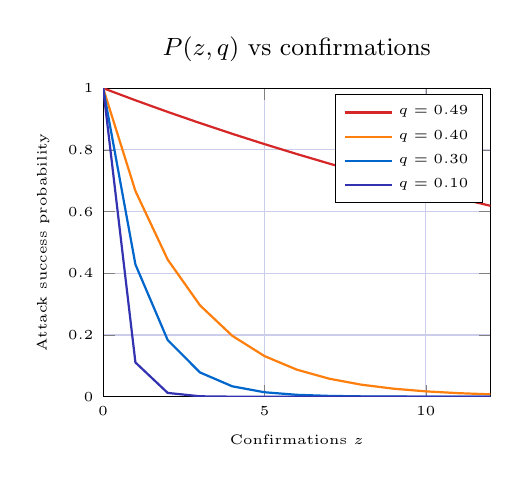
\begin{tikzpicture}
\begin{axis}[
  width=6.5cm, height=5.5cm,
  xlabel={Confirmations $z$},
  ylabel={Attack success probability},
  xmin=0,xmax=12,ymin=0,ymax=1,
  xticklabel style={font=\tiny},
  yticklabel style={font=\tiny},
  xlabel style={font=\tiny},
  ylabel style={font=\tiny},
  legend style={font=\tiny,at={(0.98,0.98)},anchor=north east},
  title={\small $P(z,q)$ vs confirmations},
  title style={font=\tiny},
  grid=major, grid style={mllavender3},
]
\addplot[mlred,thick,domain=0:12,samples=13] {0.49^x/0.51^x};
\addlegendentry{$q=0.49$}
\addplot[mlorange,thick,domain=0:12,samples=13] {(0.4/0.6)^x};
\addlegendentry{$q=0.40$}
\addplot[mlblue,thick,domain=0:12,samples=13] {(0.3/0.7)^x};
\addlegendentry{$q=0.30$}
\addplot[mlpurple,thick,domain=0:12,samples=13] {(0.1/0.9)^x};
\addlegendentry{$q=0.10$}
\end{axis}
\end{tikzpicture}
\end{columns}
\bottomnote{6 confirmations: standard for Bitcoin; $q=0.3$: $P\approx1.2\%$ after 6 blocks -- acceptable risk for most merchants}
\end{frame}

%--- FRAME 44: Attack Cost ---
\begin{frame}{51\% Attack Cost Over Time}
\begin{columns}
\column{0.55\textwidth}
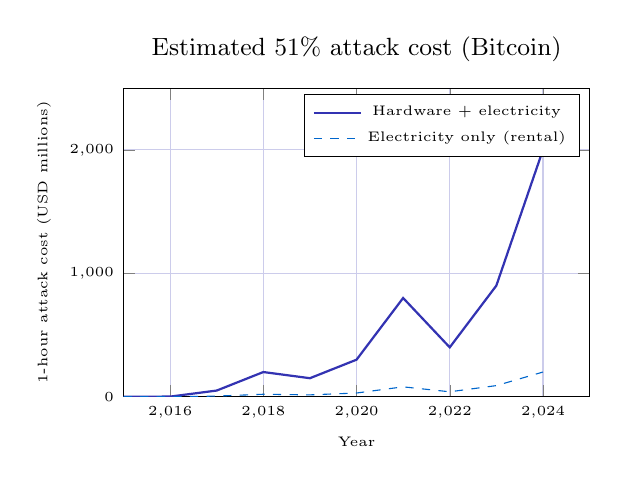
\begin{tikzpicture}
\begin{axis}[
  width=7.5cm, height=5.5cm,
  xlabel={Year},
  ylabel={1-hour attack cost (USD millions)},
  xmin=2015,xmax=2025,
  ymin=0,ymax=2500,
  xticklabel style={font=\tiny},
  yticklabel style={font=\tiny},
  xlabel style={font=\tiny},
  ylabel style={font=\tiny},
  title={\small Estimated 51\% attack cost (Bitcoin)},
  title style={font=\tiny},
  grid=major, grid style={mllavender3},
  legend style={font=\tiny},
]
\addplot[mlpurple,thick] coordinates {
  (2015,0.5)(2016,1)(2017,50)(2018,200)(2019,150)
  (2020,300)(2021,800)(2022,400)(2023,900)(2024,2000)
};
\addlegendentry{Hardware + electricity}
\addplot[mlblue,dashed] coordinates {
  (2015,0.1)(2016,0.2)(2017,5)(2018,20)(2019,15)
  (2020,30)(2021,80)(2022,40)(2023,90)(2024,200)
};
\addlegendentry{Electricity only (rental)}
\end{axis}
\end{tikzpicture}
\column{0.43\textwidth}
\begin{block}{Attack Cost Formula}
\[\text{Cost}_{\text{hw}} = \frac{H}{2} \cdot \frac{P_{\text{ASIC}}}{\eta_{\text{ASIC}}}\]
\[\text{Cost}_{\text{elec}} = \frac{H}{2} \cdot E_{\text{eff}} \cdot c_{\text{elec}}\]
$H/2$: need 50\% of current hash rate\\
$P_{\text{ASIC}}$: ASIC price per TH/s\\
$E_{\text{eff}}$: J/TH efficiency
\end{block}
\vspace{2mm}
\begin{block}{Small Chain Attacks}
Crypto51.app tracks rental costs. ETC attacked in 2020: 4 attacks, cost $\sim$\$200K each; stolen $\sim$\$5M.\\
Altcoin defense: merge mining, finality checkpoints.
\end{block}
\end{columns}
\bottomnote{Bitcoin 51\% attack: $>\$2$B hardware + ongoing electricity; economically irrational (destroys attacker's own BTC holdings)}
\end{frame}

%--- FRAME 45: Byzantine Generals ---
\begin{frame}{Byzantine Fault Tolerance}
\begin{columns}
\column{0.5\textwidth}
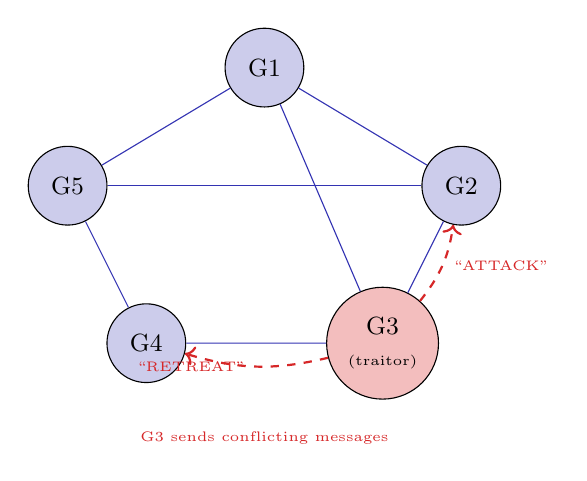
\begin{tikzpicture}[font=\small]
  \node[draw,circle,fill=mllavender3,minimum size=1cm] (g1) at (3,5) {G1};
  \node[draw,circle,fill=mllavender3,minimum size=1cm] (g2) at (5.5,3.5) {G2};
  \node[draw,circle,fill=mlred!30,minimum size=1cm,align=center] (g3) at (4.5,1.5) {G3\\\tiny(traitor)};
  \node[draw,circle,fill=mllavender3,minimum size=1cm] (g4) at (1.5,1.5) {G4};
  \node[draw,circle,fill=mllavender3,minimum size=1cm] (g5) at (0.5,3.5) {G5};
  \draw[mlpurple] (g1)--(g2)--(g3)--(g4)--(g5)--(g1);
  \draw[mlpurple] (g1)--(g3); \draw[mlpurple] (g2)--(g5);
  \draw[->,mlred,thick,dashed] (g3) to[bend right=15] node[right,font=\tiny]{``ATTACK''} (g2);
  \draw[->,mlred,thick,dashed] (g3) to[bend left=15] node[left,font=\tiny]{``RETREAT''} (g4);
  \node[font=\tiny,mlred] at (3,0.3) {G3 sends conflicting messages};
\end{tikzpicture}
\column{0.48\textwidth}
\begin{block}{Byzantine Generals Problem}
$n$ generals must agree on attack/retreat. Up to $f$ are traitors sending conflicting messages.
\end{block}
\vspace{2mm}
\begin{block}{BFT Bound}
Agreement is possible if and only if:
\[n > 3f \iff f < \frac{n}{3}\]
Requires $>2/3$ honest parties. Classic BFT (PBFT): $\mathcal{O}(n^2)$ messages.
\end{block}
\vspace{2mm}
\begin{block}{Blockchain Approach}
\small PoW/PoS replaces message complexity with economic cost. Bitcoin: probabilistic BFT. Casper: deterministic BFT with $f < n/3$.
\end{block}
\end{columns}
\bottomnote{Lamport, Shostak, Pease (1982); blockchain provides practical BFT without quadratic message complexity}
\end{frame}

%--- FRAME 46: Sybil Attack ---
\begin{frame}{Sybil Attack}
\begin{columns}
\column{0.48\textwidth}
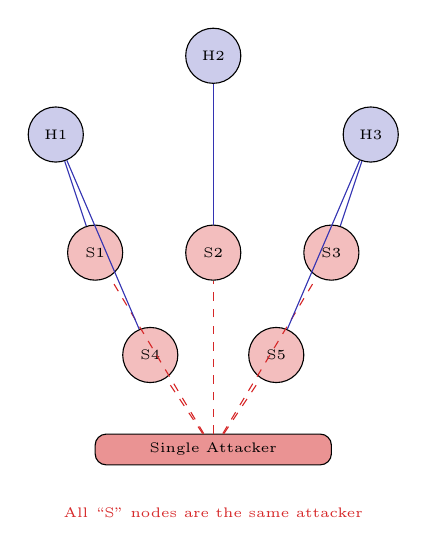
\begin{tikzpicture}[font=\tiny]
  \node[draw,circle,fill=mllavender3,minimum size=0.7cm] (h1) at (0,3) {H1};
  \node[draw,circle,fill=mllavender3,minimum size=0.7cm] (h2) at (2,4) {H2};
  \node[draw,circle,fill=mllavender3,minimum size=0.7cm] (h3) at (4,3) {H3};
  \node[draw,circle,fill=mlred!30,minimum size=0.7cm] (s1) at (0.5,1.5) {S1};
  \node[draw,circle,fill=mlred!30,minimum size=0.7cm] (s2) at (2,1.5) {S2};
  \node[draw,circle,fill=mlred!30,minimum size=0.7cm] (s3) at (3.5,1.5) {S3};
  \node[draw,circle,fill=mlred!30,minimum size=0.7cm] (s4) at (1.2,0.2) {S4};
  \node[draw,circle,fill=mlred!30,minimum size=0.7cm] (s5) at (2.8,0.2) {S5};
  \node[draw,fill=mlred!50,rounded corners,minimum width=3cm] (attacker) at (2,-1.0) {Single Attacker};
  \foreach \s in {s1,s2,s3,s4,s5} {\draw[mlred,dashed] (attacker)--(\s);}
  \foreach \h/\s in {h1/s1,h2/s2,h3/s3,h1/s4,h3/s5} {\draw[mlpurple] (\h)--(\s);}
  \node[font=\tiny,mlred] at (2,-1.8) {All ``S'' nodes are the same attacker};
\end{tikzpicture}
\column{0.50\textwidth}
\begin{block}{Sybil Attack}
Attacker creates many fake identities to gain disproportionate influence in peer selection, voting, or reputation systems.
\end{block}
\vspace{2mm}
\begin{block}{Countermeasures in Blockchain}
\begin{itemize}\small
  \item \textbf{PoW}: each identity costs computational work
  \item \textbf{PoS}: each identity costs staked capital
  \item \textbf{Eclipse attacks}: Sybil nodes surround victim, filter their view of network
  \item \textbf{Defense}: diverse peer selection, authenticated peer IDs
\end{itemize}
\end{block}
\begin{alertblock}{Eclipse Attack}\small
Attacker controls all of victim's connections $\Rightarrow$ can feed false chain, double-spend against victim.
\end{alertblock}
\end{columns}
\bottomnote{Sybil resistance: core property PoW/PoS provide; Bitcoin randomizes peer selection to resist eclipse}
\end{frame}

%--- FRAME 47: Quantum Threat ---
\begin{frame}{Quantum Computing Threats}
\begin{columns}
\column{0.5\textwidth}
\begin{block}{Grover's Algorithm}
Searches unsorted database of $N$ items in $\mathcal{O}(\sqrt{N})$.\\[4pt]
Impact on hash-based PoW:
\[\text{Classical: } \mathcal{O}(2^{256})\quad\to\quad\text{Quantum: } \mathcal{O}(2^{128})\]
SHA-256 still safe: $2^{128}$ operations beyond current/near-term quantum computers (need $\sim$$10^6$ logical qubits).
\end{block}
\vspace{2mm}
\begin{block}{Shor's Algorithm}
Factors integers in polynomial time $\mathcal{O}((\log N)^3)$.\\[4pt]
\textbf{Breaks ECDSA} (secp256k1):
\begin{itemize}\small
  \item Recovers private key from public key
  \item All coins with exposed public keys at risk
  \item P2PKH: public key only exposed on spend
  \item P2PK and reused addresses: exposed!
\end{itemize}
\end{block}
\column{0.48\textwidth}
\begin{block}{Vulnerable Bitcoin UTXOs}
\begin{tabular}{ll}
\toprule
\textbf{Type} & \textbf{Risk}\\
\midrule
P2PK & High (pubkey in UTXO)\\
Reused P2PKH & High (pubkey seen)\\
Fresh P2PKH & Medium (hash only)\\
P2WPKH & Low (hash until spend)\\
\bottomrule
\end{tabular}
$\sim$25\% of BTC supply in vulnerable addresses.
\end{block}
\vspace{2mm}
\begin{block}{Post-Quantum Candidates}
\begin{itemize}\small
  \item NIST PQC: CRYSTALS-Dilithium (signatures)
  \item Hash-based: SPHINCS+ (stateless)
  \item Timeline: migration needed before quantum threat materializes ($\sim$2030--2040?)
\end{itemize}
\end{block}
\end{columns}
\bottomnote{NIST finalized first PQC standards (2024); blockchain migration will require soft/hard fork}
\end{frame}

%--- FRAME 48: Layer 2 ---
\begin{frame}{Layer 2 Scaling Solutions}
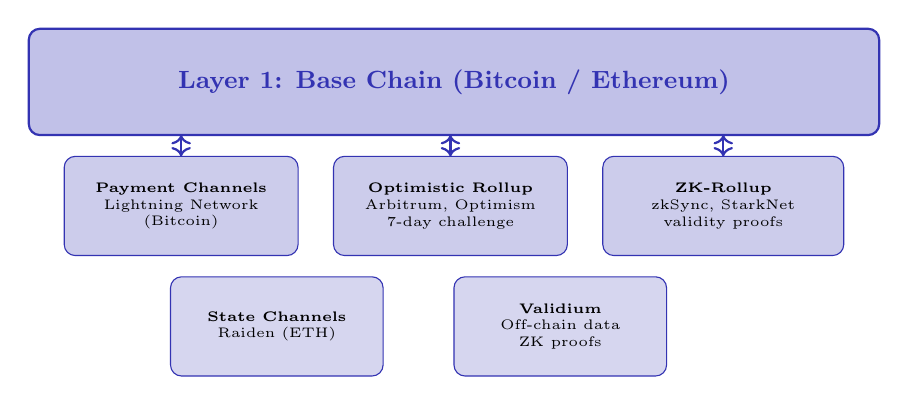
\begin{tikzpicture}[font=\small,scale=0.9]
  \draw[fill=mllavender2,draw=mlpurple,rounded corners,thick] (0,3.5) rectangle (12,5.0);
  \node[mlpurple,font=\small\bfseries] at (6,4.25) {Layer 1: Base Chain (Bitcoin / Ethereum)};
  \draw[fill=mllavender3,draw=mlpurple,rounded corners] (0.5,1.8) rectangle (3.8,3.2);
  \node[font=\tiny,align=center] at (2.15,2.5) {\textbf{Payment Channels}\\Lightning Network\\(Bitcoin)};
  \draw[fill=mllavender3,draw=mlpurple,rounded corners] (4.3,1.8) rectangle (7.6,3.2);
  \node[font=\tiny,align=center] at (5.95,2.5) {\textbf{Optimistic Rollup}\\Arbitrum, Optimism\\7-day challenge};
  \draw[fill=mllavender3,draw=mlpurple,rounded corners] (8.1,1.8) rectangle (11.5,3.2);
  \node[font=\tiny,align=center] at (9.8,2.5) {\textbf{ZK-Rollup}\\zkSync, StarkNet\\validity proofs};
  \draw[fill=mllavender4,draw=mlpurple,rounded corners] (2,0.1) rectangle (5,1.5);
  \node[font=\tiny,align=center] at (3.5,0.8) {\textbf{State Channels}\\Raiden (ETH)};
  \draw[fill=mllavender4,draw=mlpurple,rounded corners] (6,0.1) rectangle (9,1.5);
  \node[font=\tiny,align=center] at (7.5,0.8) {\textbf{Validium}\\Off-chain data\\ZK proofs};
  \draw[<->,mlpurple,thick] (2.15,3.2)--(2.15,3.5);
  \draw[<->,mlpurple,thick] (5.95,3.2)--(5.95,3.5);
  \draw[<->,mlpurple,thick] (9.8,3.2)--(9.8,3.5);
\end{tikzpicture}
\vspace{2mm}
\begin{columns}
\column{0.48\textwidth}
\begin{block}{Scalability Trilemma}
\small Blockchains struggle to simultaneously achieve: \textbf{security} + \textbf{decentralization} + \textbf{scalability}. L2 offloads computation while inheriting L1 security.
\end{block}
\column{0.48\textwidth}
\begin{block}{Throughput Comparison}
\begin{tabular}{ll}
Bitcoin L1: & $\sim$7 TPS\\
Ethereum L1: & $\sim$15 TPS\\
Lightning: & $\sim$millions TPS\\
ZK-Rollup: & $\sim$2000 TPS\\
\end{tabular}
\end{block}
\end{columns}
\bottomnote{Lightning Network: $\sim$5,000 BTC capacity (2024); ZK-rollups: fastest growing L2 category}
\end{frame}

%--- FRAME 49: Cross-Chain Bridges ---
\begin{frame}{Cross-Chain Bridges}
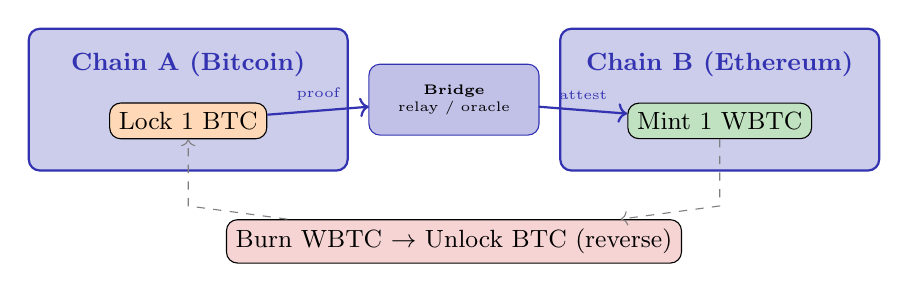
\begin{tikzpicture}[font=\small,scale=0.9]
  \draw[fill=mllavender3,draw=mlpurple,rounded corners,thick] (0,3.0) rectangle (4.5,5.0);
  \node[mlpurple,font=\small\bfseries] at (2.25,4.5) {Chain A (Bitcoin)};
  \node[draw,fill=mlorange!30,rounded corners] (lock) at (2.25,3.7) {Lock 1 BTC};
  \draw[fill=mllavender3,draw=mlpurple,rounded corners,thick] (7.5,3.0) rectangle (12,5.0);
  \node[mlpurple,font=\small\bfseries] at (9.75,4.5) {Chain B (Ethereum)};
  \node[draw,fill=mlgreen!30,rounded corners] (mint) at (9.75,3.7) {Mint 1 WBTC};
  \draw[fill=mllavender2,draw=mlpurple,rounded corners] (4.8,3.5) rectangle (7.2,4.5);
  \node[font=\tiny,align=center] at (6,4.0) {\textbf{Bridge}\\relay / oracle};
  \draw[->,mlpurple,thick] (lock)--(4.8,3.9) node[midway,above,font=\tiny]{proof};
  \draw[->,mlpurple,thick] (7.2,3.9)--(mint) node[midway,above,font=\tiny]{attest};
  \node[draw,fill=mlred!20,rounded corners,minimum width=4cm] (return) at (6,2.0) {Burn WBTC $\to$ Unlock BTC (reverse)};
  \draw[->,mlgray,dashed] (mint)--(9.75,2.5)--(return);
  \draw[->,mlgray,dashed] (return)--(2.25,2.5)--(lock);
\end{tikzpicture}
\vspace{2mm}
\begin{columns}
\column{0.5\textwidth}
\begin{block}{Bridge Types}
\begin{itemize}\small
  \item \textbf{Custodial}: centralized (WBTC, BitGo)
  \item \textbf{Optimistic}: fraud proofs, 7-day delay
  \item \textbf{ZK}: validity proofs, instant finality
  \item \textbf{Hash Time Lock}: atomic swaps (no bridge needed for 1:1 swaps)
\end{itemize}
\end{block}
\column{0.48\textwidth}
\begin{block}{Bridge Risks}
Bridges hold \$billions in TVL and are prime hack targets:
\begin{itemize}\small
  \item Ronin: \$625M (2022)
  \item Poly Network: \$611M (2021)
  \item Wormhole: \$320M (2022)
\end{itemize}
\textbf{Root cause}: oracle manipulation, key compromise, logic bugs.
\end{block}
\end{columns}
\bottomnote{Total bridge hacks (2021--2024): $>\$2$B; bridges are the weakest link in multi-chain ecosystems}
\end{frame}

%--- FRAME 51: Blockchain Interoperability ---
\begin{frame}{Blockchain Interoperability}
\begin{columns}
\column{0.5\textwidth}
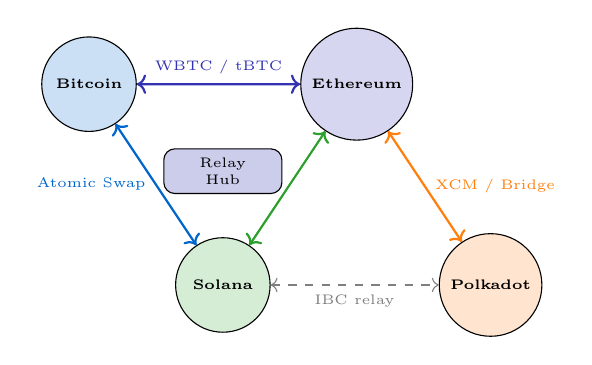
\begin{tikzpicture}[font=\tiny,scale=0.85]
  \node[draw,circle,fill=mlblue!20,minimum size=1.2cm,font=\tiny\bfseries] (btc) at (0,3.5) {Bitcoin};
  \node[draw,circle,fill=mlpurple!20,minimum size=1.2cm,font=\tiny\bfseries] (eth) at (4,3.5) {Ethereum};
  \node[draw,circle,fill=mlgreen!20,minimum size=1.2cm,font=\tiny\bfseries] (sol) at (2,0.5) {Solana};
  \node[draw,circle,fill=mlorange!20,minimum size=1.2cm,font=\tiny\bfseries] (dot) at (6,0.5) {Polkadot};
  % Interop methods
  \draw[mlpurple,thick,<->] (btc)--(eth) node[midway,above,font=\tiny]{WBTC / tBTC};
  \draw[mlgreen,thick,<->] (eth)--(sol) node[midway,left,font=\tiny]{Wormhole};
  \draw[mlblue,thick,<->] (btc)--(sol) node[midway,left,font=\tiny]{Atomic Swap};
  \draw[mlorange,thick,<->] (eth)--(dot) node[midway,right,font=\tiny]{XCM / Bridge};
  \draw[mlgray,dashed,<->] (sol)--(dot) node[midway,below,font=\tiny]{IBC relay};
  % Hub
  \node[draw,fill=mllavender3,rounded corners,minimum width=1.5cm,font=\tiny,align=center] at (2,2.2) {Relay\\Hub};
\end{tikzpicture}
\column{0.48\textwidth}
\begin{block}{Interoperability Mechanisms}
\begin{itemize}\small
  \item \textbf{Atomic Swaps}: HTLC-based trustless exchange across chains
  \item \textbf{Wrapped Tokens}: custodial (WBTC) or decentralized (tBTC)
  \item \textbf{Relay Chains}: Polkadot parachains, Cosmos IBC
  \item \textbf{Message Passing}: LayerZero, Axelar, Chainlink CCIP
\end{itemize}
\end{block}
\vspace{2mm}
\begin{block}{Atomic Swap Protocol (HTLC)}
\begin{enumerate}\small
  \item Alice creates hash lock $h = H(s)$ on Chain A
  \item Bob locks funds with same $h$ on Chain B
  \item Alice reveals secret $s$ to claim on Chain B
  \item Bob uses $s$ to claim on Chain A
  \item Timeout: refund if incomplete
\end{enumerate}
\end{block}
\end{columns}
\bottomnote{Interoperability is the ``TCP/IP moment'' for blockchains -- enabling composability across isolated networks}
\end{frame}

%--- FRAME 52: Smart Contract Platforms Comparison ---
\begin{frame}{Smart Contract Platforms Comparison}
\begin{center}
\small
\adjustbox{max width=\textwidth}{%
\begin{tabular}{lllll}
\toprule
\textbf{Feature} & \textbf{Ethereum} & \textbf{Solana} & \textbf{Cardano} & \textbf{Polkadot} \\
\midrule
\textbf{Consensus} & PoS (Casper) & PoH + Tower BFT & Ouroboros PoS & NPoS (GRANDPA) \\
\textbf{TPS (L1)} & $\sim$15--30 & $\sim$4{,}000+ & $\sim$250 & $\sim$1{,}000 \\
\textbf{Finality} & $\sim$12 min & $\sim$0.4 s & $\sim$20 s & $\sim$12--60 s \\
\textbf{VM / Lang} & EVM / Solidity & SVM / Rust & Plutus / Haskell & Wasm / Rust \\
\textbf{Fee model} & EIP-1559 (dynamic) & Fixed low fees & Predictable & Weight-based \\
\textbf{Smart contract} & Account-based & Account-based & eUTXO-based & Pallet-based \\
\textbf{Validator count} & $\sim$900{,}000+ & $\sim$1{,}900 & $\sim$3{,}200 & $\sim$300 \\
\textbf{Scaling} & L2 rollups & Firedancer & Hydra (L2) & Parachains \\
\textbf{TVL (2024)} & $\sim$\$60B & $\sim$\$5B & $\sim$\$500M & $\sim$\$300M \\
\bottomrule
\end{tabular}
}%
\end{center}
\vspace{2mm}
\begin{columns}
\column{0.48\textwidth}
\begin{block}{\textcolor{mlblue}{Design Philosophy Tradeoffs}}
\begin{itemize}\small
  \item \textbf{Ethereum}: maximum decentralization, L2-centric roadmap
  \item \textbf{Solana}: raw throughput via hardware requirements
  \item \textbf{Cardano}: formal verification, peer-reviewed research
  \item \textbf{Polkadot}: shared security via relay chain
\end{itemize}
\end{block}
\column{0.48\textwidth}
\begin{block}{\textcolor{mlpurple}{Blockchain Trilemma Position}}
\begin{itemize}\small
  \item All platforms trade off \textbf{decentralization}, \textbf{security}, and \textbf{scalability}
  \item Ethereum favors decentralization + security
  \item Solana favors scalability + security
  \item No platform achieves all three at L1
\end{itemize}
\end{block}
\end{columns}
\bottomnote{Platform choice depends on application requirements; Ethereum dominates by TVL and developer ecosystem (2024)}
\end{frame}

%--- FRAME 53: Real-World Blockchain Applications in Finance ---
\begin{frame}{Real-World Blockchain Applications in Finance}
\begin{columns}
\column{0.48\textwidth}
\begin{block}{Central Bank Digital Currencies (CBDCs)}
\begin{itemize}\small
  \item \textbf{Digital Yuan (e-CNY)}: live since 2022, 260M+ users
  \item \textbf{Digital Euro}: ECB piloting (2024--2025)
  \item Wholesale vs.\ retail CBDC designs
  \item Programmable money: conditional payments, expiry
\end{itemize}
\end{block}
\vspace{2mm}
\begin{block}{Decentralized Finance (DeFi)}
\begin{itemize}\small
  \item \textbf{DEXs}: Uniswap, Curve -- \$billions daily volume
  \item \textbf{Lending}: Aave, Compound -- algorithmic interest rates
  \item \textbf{Stablecoins}: USDC, DAI -- \$150B+ market cap
  \item Total DeFi TVL: $\sim$\$90B (2024)
\end{itemize}
\end{block}
\column{0.48\textwidth}
\begin{block}{Tokenization of Real-World Assets (RWA)}
\begin{itemize}\small
  \item \textbf{Securities}: tokenized bonds (EIB, Goldman Sachs)
  \item \textbf{Real estate}: fractional ownership via NFTs
  \item \textbf{Commodities}: Paxos Gold (PAXG), tokenized carbon credits
  \item BlackRock BUIDL fund: \$500M+ tokenized treasuries
\end{itemize}
\end{block}
\vspace{2mm}
\begin{block}{Institutional Adoption}
\begin{itemize}\small
  \item Bitcoin ETFs: \$50B+ AUM (approved Jan 2024)
  \item JPMorgan Onyx: blockchain-based payments
  \item SWIFT: CBDC interoperability experiments
  \item BIS Innovation Hub: Project mBridge (multi-CBDC)
\end{itemize}
\end{block}
\end{columns}
\bottomnote{Blockchain in finance: from fringe experiment to institutional infrastructure; RWA tokenization projected at \$16T by 2030}
\end{frame}

%--- FRAME 53: Summary ---
\begin{frame}{Summary: Key Formulas Reference Sheet}
\begin{columns}
\column{0.5\textwidth}
\begin{block}{Block \& Consensus}
\begin{tabular}{ll}
\toprule
Mining condition & $H(\text{hdr}\|\text{nonce})<T$\\
Difficulty & $D=T_{\max}/T$\\
Expected hashes & $E[N]=D\cdot 2^{32}$\\
Block reward & $R(n)=50/2^n$ BTC\\
Supply cap & $\sum 210K\cdot R(n)=21M$\\
Difficulty adj. & $D_{\text{new}}=D_{\text{old}}\cdot t_{\text{act}}/t_{\text{tgt}}$\\
\bottomrule
\end{tabular}
\end{block}
\vspace{2mm}
\begin{block}{Hash \& Merkle}
\begin{tabular}{ll}
\toprule
Birthday bound & $k\approx 2^{n/2}$ for 50\% collision\\
Proof size & $\lceil\log_2 n\rceil$ hashes\\
PoS selection & $P(i)=s_i/\sum s_j$\\
\bottomrule
\end{tabular}
\end{block}
\column{0.48\textwidth}
\begin{block}{Security \& Network}
\begin{tabular}{ll}
\toprule
51\% attack & $P(z,q)=(q/(1-q))^z$\\
BFT bound & $n>3f$\\
Nakamoto coeff. & $\min k:\sum_{i=1}^k s_i>0.5$\\
Gini & $G=\frac{\sum|s_i-s_j|}{2n\sum s_i}$\\
Entropy & $H=-\sum p_i\log_2 p_i$\\
Propagation & $t\approx\frac{\log N}{\log k}\cdot t_{\text{hop}}$\\
\bottomrule
\end{tabular}
\end{block}
\vspace{2mm}
\begin{alertblock}{Core Insight}
\small Blockchain: replace trust in institutions with cryptographic proofs + game-theoretic incentives + decentralized consensus.
\end{alertblock}
\end{columns}
\bottomnote{All formulas derived in-lecture; see Bitcoin whitepaper (Nakamoto 2008) and Ethereum Yellow Paper (Wood 2014)}
\end{frame}

\end{document}
